%                                                                 aa.dem
% AA vers. 9.1, LaTeX class for Astronomy & Astrophysics
% demonstration file
%                                                       (c) EDP Sciences
%-----------------------------------------------------------------------
%
% \documentclass[referee]{aa} % for a referee version
%\documentclass[onecolumn]{aa} % for a paper on 1 column  
%\documentclass[longauth]{aa} % for the long lists of affiliations 
%\documentclass[letter]{aa} % for the letters 
%\documentclass[bibyear]{aa} % if the references are not structured 
%                              according to the author-year natbib style

%

\documentclass[twocolumn]{aa}  

%
\usepackage{graphicx}
\usepackage{amsmath,amsfonts,amssymb}
\usepackage{natbib}
\usepackage{tabularx}
\usepackage{collcell}
\usepackage{array}
\usepackage{booktabs}
\usepackage{subfigure}
%%%%%%%%%%%%%%%%%%%%%%%%%%%%%%%%%%%%%%%%
\usepackage{txfonts}
\usepackage{xcolor}
\usepackage{blindtext}
%%%%%%%%%%%%%%%%%%%%%%%%%%%%%%%%%%%%%%%%
% \usepackage[options]{hyperref}
% To add links in your PDF file, use the package "hyperref"
% with options according to your LaTeX or PDFLaTeX drivers.
\usepackage{float}
%\usepackage{stfloats}
\usepackage{dblfloatfix}
\usepackage{afterpage}
\usepackage{ifthen}
\usepackage[morefloats=12]{morefloats}
\usepackage{tabularx}
\usepackage{placeins}
\usepackage{multicol}
%\usepackage[breaklinks,colorlinks,citecolor=blue]{hyperref}
\bibpunct{(}{)}{;}{a}{}{,}
\usepackage[switch]{lineno}
\definecolor{linkcolor}{rgb}{0.6,0,0}
\definecolor{citecolor}{rgb}{0,0,0.75}
\definecolor{urlcolor}{rgb}{0.12,0.46,0.7}
\usepackage[breaklinks, colorlinks, urlcolor=urlcolor,
linkcolor=linkcolor,citecolor=citecolor,pdfencoding=auto]{hyperref}
\hypersetup{linktocpage}
\usepackage{bold-extra}
\usepackage{ifthen}
%Planck style file, to be used with A&A style to produce Planck papers for publication.
%
% version 28 September 2010 --- useful macros --- CRL
% version 17 October 2010   --- first cut at important instrument values, from Daniele Mennella and
%                               Francois Bouchet, 13 October 2010 --- CRL
% version 18 October 2010   --- LFI FWHM changed to one value per feed, rather than M & S separately
%                               LFI FWHM uncertainties added for individual feeds.  Corrections made
%                               to LFI values. --- Andrea Zacchei
% version 24 October 2010   --- added to and corrected definitions.  No changes made to instrument
%                               quantities. --- CRL 
% version 31 October 2010   --- added definition of \muKHz. --- CRL
%
% version 15 November 2010  --- fixed conflict with aa.cls in definition of \endtable
%                               by naming the command below "\endPlancktable".  See section
%                               13.16 of the Style Guide.
%
% version 06 December 2010  --- Set up names with and without units.
%                               Add \allearlypapers command to ensure that all early papers are
%                               included in the reference list.
%                               Define macro for the name of the 4He JT cooler.
%
% version 07 December 2010  --- removed extraneous "planck2011-1.2" entry in \allearlypapers
%
% version 12 December 2010  --- added \endPlancktablewide command to set tablenotes to the full
%                               page width in the \begin{table*}...\end{table*} environment when
%                               the ``twocolumn'' option is specified in the \documentclass command.
%                               (It would be more elegant to extract the appropriate width from the
%                               aa.cls system at the time of execution, but that is buried more
%                               deeply in the system than I investigated.)
%
% version 05 January 2011   --- added unit \MJysr.  HFI performance values updated per FRB email
%                               01/05/2011 02:38-0800, and Brendan Crill email 01/05/2011 18:08 -0800.
%
% version 06 January 2011   --- changed \scriptscriptstyle primes to \scriptstyle, to better match the
%                               tx fonts used by A&A.
%
% version 07 January 2011   --- modified \allearlypapers to correspond with final early paper list.  
%                               Fixed 545 GHz center frequency.
%
% version 07 January 2011b  --- changed LFI white-noise sensitivity numbers to correct problem with units
%
% version 05 July 2011      --- added \Msol and \Lsol to get the symbols for solar mass and luminosity.
%                               Deleted previous definitions of \solar and \sol, which were equivalent
%                               to the new \Msol.
%
% version 16 August 2011    --- changed comments on \endPlancktable and \endPlancktablewide for clarity
%
% version 11 September 2011 --- changed definition of \tablenote to make footnote labels italic, as per A\&A
%
% version 26 April 2011     --- changed definition of \Planck to agree with what is said in the Style Guide (!)
%
% version 04 Dec 2013       --- included 2013 results references
%
% version 17 Jan 2014       --- included fix to bibtex file v4.3, i.e. \providecommand{\sorthelp}[1]{}
%
% version 26 Jul 2014       --- fixed incompatibility problem with aa.cls v8.0 and v8.2.  v8.2 should now be used
%                               for all Planck papers.
%                           --- fixed problem in definition of "\all2013resultspapers" that introduced a blanck
%                               into the reference to p06b.
%                           --- removed all the parameter definition stuff at the end.  We weren't using it, and
%                               it took up a lot of space.
%
% version 28 Jan 2015       --- added "\alltwentyfiftennresultspapers" and corrected "\all2013resultspapers" to
%                               "\all20thirteenresultspapers",
%
% Usage:  after the \documentclass[traditabstract]{aa} command in the La\TeX\ input file,
%         add this command:      \input Planck.tex


\def\setsymbol#1#2{\expandafter\def\csname #1\endcsname{#2}}
\def\getsymbol#1{\csname #1\endcsname}

%-----------------------------------------------------------------------
% Planck
%-----------------------------------------------------------------------
\def\Planck{\textit{Planck}}

%-----------------------------------------------------------------------
% The Planck Helium-4 JT cooler
%-----------------------------------------------------------------------
\def\HeJT{$^4$He-JT}

%-----------------------------------------------------------------------
% To include all Planck Early Results papers in the reference lists
%-----------------------------------------------------------------------
\def\allearlypapers{\nocite{planck2011-1.1, planck2011-1.3, planck2011-1.4, planck2011-1.5, planck2011-1.6, planck2011-1.7, planck2011-1.10, planck2011-1.10sup, planck2011-5.1a, planck2011-5.1b, planck2011-5.2a, planck2011-5.2b, planck2011-5.2c, planck2011-6.1, planck2011-6.2, planck2011-6.3a, planck2011-6.4a, planck2011-6.4b, planck2011-6.6, planck2011-7.0, planck2011-7.2, planck2011-7.3, planck2011-7.7a, planck2011-7.7b, planck2011-7.12, planck2011-7.13}}

%-----------------------------------------------------------------------
% To include all Planck 2013 Results papers in the reference lists
%-----------------------------------------------------------------------
\def\alltwentythirteenresultspapers{\nocite{planck2013-p01, planck2013-p02, planck2013-p02a, planck2013-p02d, planck2013-p02b, planck2013-p03, planck2013-p03c, planck2013-p03f, planck2013-p03d, planck2013-p03e, planck2013-p01a, planck2013-p06, planck2013-p03a, planck2013-pip88, planck2013-p08, planck2013-p11, planck2013-p12, planck2013-p13, planck2013-p14, planck2013-p15, planck2013-p05b, planck2013-p17, planck2013-p09, planck2013-p09a, planck2013-p20, planck2013-p19, planck2013-pipaberration, planck2013-p05, planck2013-p05a, planck2013-pip56, planck2013-p06b, planck2013-p01a}}

%-----------------------------------------------------------------------
% To include all Planck 2015 Results papers in the reference lists
%-----------------------------------------------------------------------
\def\alltwentyfifteenresultspapers{\nocite{planck2014-a01, planck2014-a03, planck2014-a04, planck2014-a05, planck2014-a06, planck2014-a07, planck2014-a08, planck2014-a09, planck2014-a11, planck2014-a12, planck2014-a13, planck2014-a14, planck2014-a15, planck2014-a16, planck2014-a17, planck2014-a18, planck2014-a19, planck2014-a20, planck2014-a22, planck2014-a24, planck2014-a26, planck2014-a28, planck2014-a29, planck2014-a30, planck2014-a31, planck2014-a35, planck2014-a36, planck2014-a37, planck2014-ES}}

%-----------------------------------------------------------------------
% Tables
%-----------------------------------------------------------------------
\newbox\tablebox    \newdimen\tablewidth
\def\leaderfil{\leaders\hbox to 5pt{\hss.\hss}\hfil}
%
% use the following definition of \endPlancktable for ApJ style notes to tables, set to the 
%         width of the table
% \def\endPlancktable{\tablewidth=\wd\tablebox 
%
% use the following definitions of \endPlancktable and \endPlancktablewide for A&A style notes 
% set to one-column  or full-page width, respectively
\def\endPlancktable{\tablewidth=\columnwidth 
    $$\hss\copy\tablebox\hss$$
    \vskip-\lastskip\vskip -2pt}
\def\endPlancktablewide{\tablewidth=\textwidth 
    $$\hss\copy\tablebox\hss$$
    \vskip-\lastskip\vskip -2pt}
\def\tablenote#1 #2\par{\begingroup \parindent=0.8em
    \abovedisplayshortskip=0pt\belowdisplayshortskip=0pt
    \noindent
    $$\hss\vbox{\hsize\tablewidth \hangindent=\parindent \hangafter=1 \noindent
    \hbox to \parindent{$^#1$\hss}\strut#2\strut\par}\hss$$
    \endgroup}
\def\doubleline{\vskip 3pt\hrule \vskip 1.5pt \hrule \vskip 5pt}

%-----------------------------------------------------------------------
% useful macros
%-----------------------------------------------------------------------
%
\def\L2{\ifmmode L_2\else $L_2$\fi}
%
\def\dtt{\Delta T/T}
\def\DeltaT{\ifmmode \Delta T\else $\Delta T$\fi}
\def\deltat{\ifmmode \Delta t\else $\Delta t$\fi}
\def\fknee{\ifmmode f_{\rm knee}\else $f_{\rm knee}$\fi}
\def\Fmax{\ifmmode F_{\rm max}\else $F_{\rm max}$\fi}
%
\def\solar{\ifmmode{\rm M}_{\mathord\odot}\else${\rm M}_{\mathord\odot}$\fi}
\def\Msolar{\ifmmode{\rm M}_{\mathord\odot}\else${\rm M}_{\mathord\odot}$\fi}
\def\Lsolar{\ifmmode{\rm L}_{\mathord\odot}\else${\rm L}_{\mathord\odot}$\fi}
%
\def\inv{\ifmmode^{-1}\else$^{-1}$\fi}
\def\mo{\ifmmode^{-1}\else$^{-1}$\fi}
\def\sup#1{\ifmmode ^{\rm #1}\else $^{\rm #1}$\fi}
\def\expo#1{\ifmmode \times 10^{#1}\else $\times 10^{#1}$\fi}
%
\def\,{\thinspace}
\def\lsim{\mathrel{\raise .4ex\hbox{\rlap{$<$}\lower 1.2ex\hbox{$\sim$}}}}
\def\gsim{\mathrel{\raise .4ex\hbox{\rlap{$>$}\lower 1.2ex\hbox{$\sim$}}}}
\let\lea=\lsim
\let\gea=\gsim
\def\simprop{\mathrel{\raise .4ex\hbox{\rlap{$\propto$}\lower 1.2ex\hbox{$\sim$}}}}
%
\def\deg{\ifmmode^\circ\else$^\circ$\fi}
\def\pdeg{\ifmmode $\setbox0=\hbox{$^{\circ}$}\rlap{\hskip.11\wd0 .}$^{\circ}
          \else \setbox0=\hbox{$^{\circ}$}\rlap{\hskip.11\wd0 .}$^{\circ}$\fi}
\def\arcs{\ifmmode {^{\scriptstyle\prime\prime}}
          \else $^{\scriptstyle\prime\prime}$\fi}
\def\arcm{\ifmmode {^{\scriptstyle\prime}}
          \else $^{\scriptstyle\prime}$\fi}
\newdimen\sa  \newdimen\sb
\def\parcs{\sa=.07em \sb=.03em
     \ifmmode \hbox{\rlap{.}}^{\scriptstyle\prime\kern -\sb\prime}\hbox{\kern -\sa}
     \else \rlap{.}$^{\scriptstyle\prime\kern -\sb\prime}$\kern -\sa\fi}
\def\parcm{\sa=.08em \sb=.03em
     \ifmmode \hbox{\rlap{.}\kern\sa}^{\scriptstyle\prime}\hbox{\kern-\sb}
     \else \rlap{.}\kern\sa$^{\scriptstyle\prime}$\kern-\sb\fi}
%
\def\ra[#1 #2 #3.#4]{#1\sup{h}#2\sup{m}#3\sup{s}\llap.#4}
\def\dec[#1 #2 #3.#4]{#1\deg#2\arcm#3\arcs\llap.#4}
\def\deco[#1 #2 #3]{#1\deg#2\arcm#3\arcs}
\def\rra[#1 #2]{#1\sup{h}#2\sup{m}}
%
\def\page{\vfill\eject}
\def\dots{\relax\ifmmode \ldots\else $\ldots$\fi}
%
%-----------------------------------------------------------------------
% units
%-----------------------------------------------------------------------
%
\def\WHzsr{\ifmmode $W\,Hz\mo\,sr\mo$\else W\,Hz\mo\,sr\mo\fi}
\def\mHz{\ifmmode $\,mHz$\else \,mHz\fi}
\def\GHz{\ifmmode $\,GHz$\else \,GHz\fi}
\def\mKs{\ifmmode $\,mK\,s$^{1/2}\else \,mK\,s$^{1/2}$\fi}
\def\muKs{\ifmmode \,\mu$K\,s$^{1/2}\else \,$\mu$K\,s$^{1/2}$\fi}
\def\muKRJs{\ifmmode \,\mu$K$_{\rm RJ}$\,s$^{1/2}\else \,$\mu$K$_{\rm RJ}$\,s$^{1/2}$\fi}
\def\muKHz{\ifmmode \,\mu$K\,Hz$^{-1/2}\else \,$\mu$K\,Hz$^{-1/2}$\fi}
\def\MJysr{\ifmmode \,$MJy\,sr\mo$\else \,MJy\,sr\mo\fi}
\def\MJysrmK{\ifmmode \,$MJy\,sr\mo$\,mK$_{\rm CMB}\mo\else \,MJy\,sr\mo\,mK$_{\rm CMB}\mo$\fi}
\def\microns{\ifmmode \,\mu$m$\else \,$\mu$m\fi}
\def\micron{\microns}
\def\muK{\ifmmode \,\mu$K$\else \,$\mu$\hbox{K}\fi}
\def\microK{\ifmmode \,\mu$K$\else \,$\mu$\hbox{K}\fi}
\def\muW{\ifmmode \,\mu$W$\else \,$\mu$\hbox{W}\fi}
\def\kms{\ifmmode $\,km\,s$^{-1}\else \,km\,s$^{-1}$\fi}
\def\kmsMpc{\ifmmode $\,\kms\,Mpc\mo$\else \,\kms\,Mpc\mo\fi}
%
%
%----------------------------------------------------------------------
% set up machinery to list Planck papers in roman numeral order.
%----------------------------------------------------------------------

\providecommand{\sorthelp}[1]{}


% Custom definitions
\def\Cosmoglobe{\textsc{Cosmoglobe}}
\def\commander{\texttt{Commander}}
\def\commanderthree{\texttt{Commander3}}
\def\Commander{\texttt{Commander}}
\def\Planck{\textit{Planck}}
\def\WMAP{\textit{WMAP}}
\def\Spitzer{\textit{Spitzer}}
\def\Gaia{\textit{Gaia}}

\newcommand{\cii}{\ensuremath{\mathsc {C\ ii}}}

\newcommand{\nWmsr}{\mathrm{nW}\,\mathrm{m}^{-2}\,\mathrm{sr}^{-1}}
\newcommand{\um}{$\,\mu\mathrm{m}$}
\newcommand{\phm}{\phantom{-}}
\newcommand{\dv}[0]{\vec{d}}
\renewcommand{\t}[0]{\vec{t}}
\newcommand{\A}[0]{\tens{A}}
\newcommand{\B}[0]{\tens{B}}
\newcommand{\Y}[0]{\tens{Y}}
\newcommand{\n}[0]{\vec{n}}
\newcommand{\red}[0]{\color{red}}
\newcommand{\green}[0]{\color{green}}
\newcommand{\s}[0]{\vec{s}}
\renewcommand{\a}[0]{\vec{a}}
\newcommand{\m}[0]{\vec{m}}
\newcommand{\bv}[0]{\vec{b}}
\newcommand{\f}[0]{\vec{f}}
\newcommand{\F}[0]{\tens{F}}
\newcommand{\T}[0]{\tens{T}}
\newcommand{\Cp}[0]{\tens{C}}
\renewcommand{\L}[0]{\tens{L}}
\newcommand{\g}[0]{\vec{g}}
\newcommand{\N}[0]{\tens{N}}
\newcommand{\M}[0]{\tens{M}}
\newcommand{\iN}[0]{\tens{N}^{-1}}
\newcommand{\iM}[0]{\tens{M}^{-1}}
\newcommand{\w}[0]{\vec{w}}
\renewcommand{\S}[0]{\tens{S}}
\renewcommand{\r}[0]{\vec{r}}
\renewcommand{\u}[0]{\vec{u}}
\newcommand{\q}[0]{\vec{q}}
\renewcommand{\v}[0]{\vec{v}}
\renewcommand{\P}[0]{\tens{P}}
\newcommand{\dt}[0]{d_t}
\newcommand{\di}[0]{d_i}
\newcommand{\nt}[0]{n_t}
\newcommand{\st}[0]{s_t}
\newcommand{\mt}[0]{m_t}
\newcommand{\ft}[0]{f_t}
\newcommand{\Te}[0]{T_{\rm e}}
\newcommand{\EM}[0]{\rm EM}
\newcommand{\mathsc}[1]{{\normalfont\textsc{#1}}}
\newcommand{\hi}{\ensuremath{\mathsc {H\ i}}}
\newcommand{\bpbold}{\bfseries{\scshape{BeyondPlanck}}}
\newcommand{\BP}{\textsc{BeyondPlanck}}
\newcommand{\bp}{\textsc{BeyondPlanck}}
\newcommand{\cosmoglobe}{\textsc{Cosmoglobe}}
%\newcommand{\Cosmoglobe}{\textsc{Cosmoglobe}}
\newcommand{\lfi}[0]{LFI}
\newcommand{\hfi}[0]{HFI}
\newcommand{\npipe}[0]{\texttt{NPIPE}}
\newcommand{\K}[0]{\textit K}
\newcommand{\Ka}[0]{\textit{Ka}}
\newcommand{\Q}[0]{\textit Q}
\newcommand{\V}[0]{\textit V}
\newcommand{\W}[0]{\textit W}
\newcommand{\e}{\mathrm e}
\newcommand{\cvar}{\ensuremath{c(\vartheta, \varphi, \psi)}}


\def\Tcmb{\ifmmode T_\mathrm{CMB}\else $T_{\mathrm{CMB}}$\fi}
\def\Tcold{\ifmmode T_\mathrm{c}\else $T_{\mathrm{c}}$\fi}
\def\Thot{\ifmmode T_\mathrm{h}\else $T_{\mathrm{h}}$\fi}
\def\Tnear{\ifmmode T_\mathrm{n}\else $T_{\mathrm{n}}$\fi}
\def\scmb{\ifmmode s_\mathrm{CMB}\else $s_{\mathrm{CMB}}$\fi}
\def\squad{\ifmmode s_\mathrm{quad}\else $s_{\mathrm{quad}}$\fi}
\def\ssynch{\ifmmode s_\mathrm{s}\else $s_\mathrm{s}$\fi}
\def\sdust{\ifmmode s_\mathrm{d}\else $s_{\mathrm{d}}$\fi}
\def\ssdust{\ifmmode s_\mathrm{sd}\else $s_{\mathrm{sd}}$\fi}
\def\same{\ifmmode s_\mathrm{AME}\else $s_{\mathrm{AME}}$\fi}
\def\ssrc{\ifmmode s_\mathrm{src}\else $s_{\mathrm{src}}$\fi}
\def\sco{\ifmmode s_\mathrm{CO}\else $s_{\mathrm{CO}}$\fi}
\def\sff{\ifmmode s_\mathrm{ff}\else $s_{\mathrm{ff}}$\fi}
\def\gff{\ifmmode g_\mathrm{ff}\else $g_{\mathrm{ff}}$\fi}
\def\fsynch{\ifmmode f_\mathrm{s}\else $f_{\mathrm{s}}$\fi}
\def\fsd{\ifmmode f_\mathrm{sd}\else $f_{\mathrm{sd}}$\fi}
\def\fame{\ifmmode f_\mathrm{AME}\else $f_{\mathrm{AME}}$\fi}
\def\alphasrc{\ifmmode \alpha_\mathrm{src}\else $\alpha_{\mathrm{src}}$\fi}
\def\bcold{\ifmmode \beta_\mathrm{c}\else $\beta_{\mathrm{c}}$\fi}
\def\bhot{\ifmmode \beta_\mathrm{h}\else $\beta_{\mathrm{h}}$\fi}
\def\bnear{\ifmmode \beta_\mathrm{n}\else $\beta_{\mathrm{n}}$\fi}
\def\bsynch{\ifmmode \beta_\mathrm{s}\else $\beta_{\mathrm{s}}$\fi} 
\def\bsun{\ifmmode \beta_\mathrm{sun}\else $\beta_{\mathrm{sun}}$\fi} 
\def\nuzeros{\ifmmode \nu_{0,\mathrm{s}}\else $\nu_{0,\mathrm{s}}$\fi} 
\def\nuzeroff{\ifmmode \nu_{0,\mathrm{ff}}\else $\nu_{0,\mathrm{ff}}$\fi} 
\def\nuzerocold{\ifmmode \nu_{0,\mathrm{c}}\else $\nu_{0,\mathrm{c}}$\fi}
\def\nuzerohot{\ifmmode \nu_{0,\mathrm{h}}\else $\nu_{0,\mathrm{h}}$\fi}
\def\nuzeronear{\ifmmode \nu_{0,\mathrm{n}}\else $\nu_{0,\mathrm{n}}$\fi} 
\def\nuzeroame{\ifmmode \nu_{0,\mathrm{AME}}\else $\nu_{0,\mathrm{AME}}$\fi} 
\def\nuzerosd{\ifmmode \nu_{0,\mathrm{}}\else $\nu_{0,\mathrm{sd}}$\fi} 
\def\nuzerosrc{\ifmmode \nu_{0,\mathrm{src}}\else $\nu_{0,\mathrm{src}}$\fi} 
\def\nup{\ifmmode \nu_{\mathrm{p}}\else $\nu_{\mathrm{p}}$\fi} 
\def\alphasd{\ifmmode \alpha_{\mathrm{sd}}\else $\alpha_{\mathrm{sd}}$\fi} 
\def\Te{\ifmmode T_{\mathrm{e}}\else $T_{\mathrm{e}}$\fi} 
\def\kB{\ifmmode k_\mathrm{B}\else $k_{\mathrm{B}}$\fi} 

% \renewcommand{\topfraction}{1.0}	% max fraction of floats at top
%     \renewcommand{\bottomfraction}{1.0}	% max fraction of floats at bottom
%     %   Parameters for TEXT pages (not float pages):
%     \setcounter{topnumber}{2}
%     \setcounter{bottomnumber}{2}
%     \setcounter{totalnumber}{4}     % 2 may work better
%     \setcounter{dbltopnumber}{2}    % for 2-column pages
%     \renewcommand{\dbltopfraction}{0.9}	% fit big float above 2-col. text
%     \renewcommand{\textfraction}{0.04}	% allow minimal text w. figs
%     %   Parameters for FLOAT pages (not text pages):
%     \renewcommand{\floatpagefraction}{0.9}	% require fuller float pages
% 	% N.B.: floatpagefraction MUST be less than topfraction !!
%     \renewcommand{\dblfloatpagefraction}{0.9}	% require fuller float pages



\begin{document} 

   \title{\bfseries{\Cosmoglobe\ DR2. III. Improved modelling of zodiacal light emission in \textit{COBE}-DIRBE through Bayesian global analysis}}

   %This author list corresponds to \title{Author list for L04\_CMB\_Foregrounds\_Extraction}
%Prepared by M. Lopez-Caniego (Marcos.Lopez.Caniego@sciops.esa.int), ESAC/ESA
%This version is from Thu Jul 12 18:11:48 2018 CET
%\subtitle{There are 152 co-authors in this list}
\newcommand{\oslo}[0]{1}
\newcommand{\iiabangalore}[0]{2}

\author{\small
D.~J.~Watts\inst{\ref{uio}}\thanks{Corresponding author: D.~J.~Watts; \url{duncanwa@astro.uio.no}}
\and
A.~Basyrov\inst{\ref{uio}}
\and
H.~T.~Ihle\inst{\ref{uio}}
\and
S.~Paradiso\inst{\ref{waterloo}}
\and
F.~Rahman\inst{\ref{iiabangalore}}
\and
H.~Thommesen\inst{\ref{uio}}
\and
M.~Bersanelli\inst{\ref{milan}}
\and
L.~A.~Bianchi\inst{\ref{milan}}
\and
M.~Brilenkov\inst{\ref{uio}}
\and
L.~P.~L.~Colombo\inst{\ref{milan}}
\and
H.~K.~Eriksen\inst{\ref{uio}}
\and
J.~R.~Eskilt\inst{\ref{uio},\ref{imperial}}
\and
K.~S.~F.~Fornazier\inst{\ref{saopaulo}}
\and
C.~Franceschet\inst{\ref{milan}}
\and
U.~Fuskeland\inst{\ref{uio}}
\and
M.~Galloway\inst{\ref{uio}}
\and
E.~Gjerl\o w\inst{\ref{uio}}
\and
B.~Hensley\inst{\ref{princeton}}
\and
L.~T.~Hergt\inst{\ref{ubc}}
\and
D.~Herman\inst{\ref{uio}}
\and
G.~A.~Hoerning\inst{\ref{saopaulo}}
\and
K.~Lee\inst{\ref{uio}}
\and
J.~G.~S.~Lunde\inst{\ref{uio}}
\and
A.~Marins\inst{\ref{saopaulo},\ref{ustofc}}
\and
S.~K.~Nerval\inst{\ref{dunlap1},\ref{dunlap2}}
\and
S.~K.~Patel\inst{\ref{iit_bhu}}
\and
M.~Regnier\inst{\ref{apc}}
\and
M.~San\inst{\ref{uio}}
\and
S.~Sanyal\inst{\ref{iit_bhu}}
\and
N.-O.~Stutzer\inst{\ref{uio}}
\and
A.~Verma\inst{\ref{iit_bhu}}
\and
I.~K.~Wehus\inst{\ref{uio}}
\and
Y.~Zhou\inst{\ref{berkeley}}
}
\institute{\small
Institute of Theoretical Astrophysics, University of Oslo, Blindern, Oslo, Norway\label{uio}
\and
Waterloo Centre for Astrophysics, University of Waterloo, Waterloo, ON N2L 3G1, Canada\label{waterloo}
\and
Indian Institute of Astrophysics, Koramangala II Block, Bangalore, 560034, India\label{iiabangalore}
\and
Dipartimento di Fisica, Università degli Studi di Milano, Via Celoria, 16, Milano, Italy\label{milan}
\and
Imperial Centre for Inference and Cosmology, Department of Physics, Imperial College London, Blackett Laboratory, Prince Consort Road, London SW7 2AZ, United Kingdom\label{imperial}
\and
Instituto de Física, Universidade de São Paulo - C.P. 66318, CEP: 05315-970, São Paulo, Brazil\label{saopaulo}
\and
Department of Astrophysical Sciences, Princeton University, 4 Ivy Lane, Princeton, NJ 08540\label{princeton}
\and
Department of Physics and Astronomy, University of British Columbia, 6224 Agricultural Road, Vancouver BC, V6T1Z1, Canada\label{ubc}
\and
Department of Astronomy,  University of Science and Technology of China, Hefei, China\label{ustofc}
\and
David A. Dunlap Department of Astronomy \& Astrophysics, University of Toronto, 50 St. George Street, Toronto, ON M5S 3H4, Canada\label{dunlap1}
\and
Dunlap Institute for Astronomy \& Astrophysics, University of Toronto, 50 St. George Street, Toronto, ON M5S 3H4, Canada\label{dunlap2}
\and
Department of Physics, Indian Institute of Technology (BHU), Varanasi - 221005, India\label{iit_bhu}
\and
Laboratoire Astroparticule et Cosmologie (APC), Université Paris-Cité, Paris, France\label{apc}
\and
Department of Physics, UC Berkeley\label{berkeley}
}

 %\author{V.~Arsenijevic\inst{\ref{inst1}}\and S.~Fabbro\inst{\ref{inst2}}\and
%A.~M.~Mour\~ao\inst{\ref{inst3}}\and A.~J.~Rica da Silva\inst{\ref{inst1}}}
%
%\institute{Multidisciplinar de Astrof\'{\i}sica, IST, Avenida Rovisco Pais, 1049
%Lisbon, Portugal\email{...}\label{inst1} \and < Multidisciplinar de Astrof\'{\i}sica, IST, Avenida Rovisco Pais, 1049 Lisbon, Portugal\email{...}\label{inst2}
%\and
%Multidisciplinar de Astrof\'{\i}sica, IST, Avenida Rovisco Pais, 1049
%Lisbon, Portugal\email{...}\label{inst3}
%} 


   %\institute{Institute of Theoretical Astrophysics, University of Oslo, Blindern, Oslo, Norway}
  
   % Shortened title, author list for top of page 
   \titlerunning{\Cosmoglobe: Interplanetary dust}
   \authorrunning{M.~San et al.}

   \date{\today}
   

% write an abstract 

   \abstract{We present an improved model of zodiacal light (ZL) emission for \textit{COBE}-DIRBE derived through global Bayesian analysis within \cosmoglobe\ Data Release~2 (DR2). The parametric form of the ZL model is identical to that introduced by Kelsall et al. (1998; K98), but the specific best-fit parameter values are rederived using the combination of DIRBE Calibrated Individual Observations (CIOs), \Planck\ HFI sky maps, and WISE and GAIA compact object catalogs. Furthermore, the ZL parameters are fitted jointly with astrophysical parameters, such as thermal dust and starlight emission, and the new model takes into account excess radiation that appears stationary in solar-centric coordinates as reported in a companion paper. The relative differences in predicted signals at 25$\,\mu\mathrm{m}$ between K98 and our new model are $\lesssim\,2\,\%$ in the Ecliptic plane, and $\lesssim\,5\,\%$ in the Ecliptic poles and along the asteroidal bands. The zero-level of the cleaned DR2 maps are lower than those of the legacy DIRBE Zodiacal light Subtracted Mission Average (ZSMA) maps by $\sim$\,10\,kJy/sr at 1.25--3.5\,$\mu\mathrm{m}$, which is comparable to the entire predicted contribution from high-redshift galaxies to the Cosmic Infrared Background (CIB) at the same wavelengths. The total rms's of each DR2 maps at wavelengths up to and including $60\,\mu\mathrm{m}$ are $\sim$\,30\,\% lower at high Galactic latitudes than the corresponding DIRBE ZSMA maps. The cleaned DR2 maps at 4.9 and 60\,$\mu\mathrm{m}$ are now for the first time visually dominated by Galactic signal at high latitudes rather than by ZL residuals. Even the 100$\,\mu\mathrm{m}$ channel, which has served as a cornerstone for Galactic studies for three decades, appears significantly cleaner in the current processing. Still, obvious ZL residuals can be seen even in several of the DR2 maps, and further work is required to mitigate these. Joint analysis with existing and future high-resolution full-sky surveys such as AKARI, IRAS, \Planck\ HFI, and SPHEREx will be essential both to break key degeneracies in the current model and to determine whether the reported solar-centric excess radiation has a ZL or instrumental origin. On the algorithmic side, more efficient methods for probing massively multi-peaked likelihoods should be explored and implemented. Thus, while the results presented in this paper do re-define the state-of-the-art for DIRBE modelling, it also only represents the first among many steps toward a future optimal Bayesian ZL model.
}

   \keywords{Zodiacal dust, Interplanetary medium, Cosmology: cosmic background radiation}

   \maketitle

\setcounter{tocdepth}{2}
\tableofcontents
   

\section{Introduction}
Zodiacal light (ZL, sometimes zodiacal emission or interplanetary dust
emission) is the primary source of diffuse radiation observed in the
infrared sky between 1-100 $\mu$m (see, e.g., \citealp{Leinert1998}
and references therein). This radiation comes from scattering and
re-emission of sunlight from interplanetary dust (IPD) grains, and was
first mapped in detail by the IRAS satellite
\citep{neugebauer:1984}.

The inner Solar system is embedded in a Sun centered cloud of IPD,
with a symmetry axis tilted slightly with respect to the Ecliptic,
known as the zodiacal cloud. The ZL is seasonal, and its appearance in
the sky changes as the Earth moves through the IPD distribution. The
most common way to model the observer position-dependent ZL is to
evaluate a line-of-sight integral for each observation directly in the
time-ordered domain. The time-varying and three-dimensional nature of
the ZL makes it one of the most challenging foregrounds to model in
astrophysical and cosmological studies of the infrared sky. The lack
of a high-accuracy ZL model has left a large part of the
electromagnetic spectrum inaccessible to cosmological analysis
attempting to measure the Cosmic Infrared Background (CIB;
\citealp{partridge1967,hauser1998,hauser:2001}).

One of the most widely used ZL models in the field of cosmology is the
\textit{COBE}/DIRBE model by \citet{Kelsall1998}, often simply
referred to as the K98 model. This is a parametric three-dimensional
model that describes the three-dimensional IPD distribution and the
radiative properties of dust using time-dependent measurements from
the \textit{COBE}/DIRBE instrument \citep{hauser1998}. Since then, our
understanding of the infrared sky has improved with new observational
data from experiments like WISE \citep{wright:2010}, Planck HFI
\citep{planck2016-l03}, and GAIA \citep{gaia:2016}. However, these
experiments have largely been analyzed individually, and little or no
coordinated effort has been made toward combining the data from these
experiments into one overall state-of-the-art model of the infrared
sky. The main goal of the current work, summarized in a series of
papers collectively denoted \cosmoglobe\ Data Release 2, is to make
the first step toward such a concordance model by leveraging recent
computational advances in Bayesian cosmological data analysis by the
\BP\ \citep[][and references therein]{BP2023,Galloway2023} and
\cosmoglobe\ \citep{Watts2023} collaborations. The computer code
implementation is called \commanderthree\ \citep{Galloway2023}, which
is a Bayesian Gibbs sampler that was originally designed for
end-to-end analysis of cosmic microwave background (CMB) experiments,
in particular \Planck\ LFI \citep{planck2016-l02} and \WMAP
\citep{bennett2012}. However, as demonstrated in the current work, the
same algorithms are after relatively minor modifications also directly
applicable to infrared measurements.

One of the most important generalizations required for application of
\commanderthree\ to the infrared sky is the implementation of an
accurate time-variable ZL model. In this paper we therefore implement
support for the K98 model in \commanderthree, and we apply this to the
time-domain DIRBE data. This new code is based ZodiPy \citep{San2024},
which is an Astropy-affiliated Python package for ZL simulations. As
an early application of this framework, \cite{San2022} demonstrated
the removal of ZL from the DIRBE TOD with ZodiPy using the K98 model.

The rest of the paper is organized as follows. In
Sect.~\ref{sect:zodi-model}, we introduce the K98 ZL model and discuss
implementation and optimization aspects. Next, in
Sect.~\ref{sect:data}, we describe the data used in the current
analysis, before summarizing the algorithms in
Sect.~\ref{sect:param-estimation}. We present our updated ZL model and
compare this with K98 in Sect.~\ref{sect:improved-model}. Finally, we
conclude in Sect.~\ref{sec:conclusions}.


\section{Zodiacal light modelling}\label{sect:zodi-model}
ZL is commonly modelled sample-by-sample in time-domain by performing
line-of-sight integration at each observation through a parametric
three-dimensional model of the IPD distribution. We adopt the same
general parametrization as introduced by K98 for the current
\commanderthree\ implementation, and in this section we briefly review
the main aspects of this model, aiming to build intuition about the
underlying parametric model. We also consider a few numerical
approximations that reduce the overall computational cost. For full
details of this model, we refer the interested reader to
\citet{Kelsall1998}.

\subsection{Parameterization of interplanetary dust}
IPD in the zodiacal cloud is overall smooth and stable, and most of
the dust may be accounted for by a diffuse cloud-like component
\citep{Leinert1998}.  The majority of this dust stems from
mass-shedding of various Jupiter family comets with low eccentricities
and inclinations with respect to the Ecliptic. However, fine
structures within the zodiacal cloud exist as a result of collisions
and fragmentation in asteroids and gravitational resonance in the
orbit of planets \citep{Low1984, Dermott1984, Dermott1994, Reach1997}.

We model the IPD distribution as a combination of several zodiacal
components, each described by a number density $n_c(x,y,z)$, where $c$
indicates components and $x$, $y$ and $z$ indicate heliocentric
Ecliptic coordinates. Each zodiacal component is allowed to have a
heliocentric offset $(x_{0,c}, y_{0,c}, z_{0,c})$, such that the
component-centric coordinates become
\begin{equation}    
    \begin{aligned}
        x_c&= x - x_{0,c}\\
        y_c&= y - y_{0,c}\\
        z_c&= z - z_{0,c}.
    \end{aligned}
\end{equation}
Additionally, each zodiacal component is allowed to have a plane of
symmetry that is different from the Ecliptic, which is defined by an
inclination $i_c$ and an ascending node $\Omega_c$. Components that
happen to be azimuthally symmetric are then fully described by a
radial distance $r_c$ from the origin and the height above the
symmetry plane $Z_c$,
\begin{align}
    r_c &= \sqrt{x_c^2 + y_c^2 + z_c^2},\\
    Z_c &= x_c\sin{\Omega_c}\sin{i_c} - y_c \cos{\Omega_c}\sin{i_c} + z_c \cos{i_c},\\
    \zeta_c &= \frac{|Z_\mathrm{c}|}{r_\mathrm{c}},
\end{align}
where $\zeta_c$ is the radial height above the symmetry plane.

\subsection{Zodiacal components}

With these definitions in hand, we now define parametric models for
each IPD component type.

\subsubsection{Smooth cloud}
By far the most important component is typically referred to as the
``zodiacal cloud''. This component represents the smooth IPD
distribution that embeds the inner Solar system. Its number density is
modeled as
\begin{equation}
    n_\mathrm{C}(x,y,z)=n_{0,
      \mathrm{C}}r_\mathrm{C}^{-\alpha}f(\zeta_\mathrm{C}),
    \label{eq:cloud}
\end{equation}
where $n_{0, \mathrm{C}}$ is the number density at 1\,AU, $\alpha$ is a 
power-law index, $f(\zeta_\mathrm{C})$ is the fan-like vertical 
distribution given as 
\begin{equation}
    f(\zeta_\mathrm{C}) = \exp {\left[-\beta g^\gamma \right]},
\end{equation}
with
\begin{equation}
    g = \begin{cases}
        \zeta^2/2\mu & \mathrm{for}\; \zeta < \mu,\\
        \zeta - \mu/2 & \mathrm{for}\; \zeta \geq \mu,
    \end{cases}
\end{equation}
where $\beta$, $\gamma$ and $\mu$ are shape parameters.

\subsubsection{Dust bands}
Next, three dust bands are included in the model to represent the
observed shoulder-like structure in the IRAS scans across the ecliptic
plane.  These bands appear at Ecliptic latitudes of $\pm \sim
1.4^\circ$, $10^\circ$, and $15^\circ$, and are associated with the
Themis, Koronis, and Eos asteroid families, respectively ({\bf ADD
  CITATION}). Each dust band, indicated by $B_ii$, is modeled as
\begin{align}
    n_{\mathrm{B}_i}(x,y,z) &= \frac{3 n_{0, \mathrm{B}_i}}{r_{\mathrm{B}_i}} \exp \left[-\left(\frac{\zeta_{\mathrm{B}_i}}{\delta_{\zeta_{\mathrm{B}_i}}}\right)^{6}\right]\left[1 + \left(\frac{\zeta_{\mathrm{B}_i}}{\delta_{\zeta_{\mathrm{B}_i}}}\right)^{p}v^{-1}\right] \\
    &\times\left\{1-\exp \left[-\left(\frac{r_{\mathrm{B}_i}}{\delta_{r_{\mathrm{B}_i}}}\right)^{20}\right]\right\},
\label{eq:band}
\end{align}
where $n_{0, \mathrm{B}_i}$ is the number density of band $\mathrm{B}_i$ 
at 3\,AU, $\delta_{r_{\mathrm{B}_i}}$ is the inner radial cut-off, and 
$p$, $v$ and $\delta_{\zeta_{\mathrm{B}_i}}$ are shape parameters.

\subsubsection{Circum-solar ring and Earth-trailing feature}
Finally, a circum-solar ring (denoted ``SR'') component is included in the
model to represent dust that has accumulated in Earth's orbit due to
gravitational effects ({\bf ADD REFERENCE}). This component also
includes an enhancement to the IPD distribution at Earth's wake, known
as the ``Earth-trailing feature'' (denoted ``TF''). The ring component is modeled as
\begin{align}
    n_\mathrm{R}(x, y, z, \theta)&=n_{0, \mathrm{SR}} \exp \left[-\frac{\left(r_\mathrm{R}-r_{0, \mathrm{SR}}\right)^2}{\sigma_{R,\mathrm{SR}} ^2}-\frac{\left| Z_\mathrm{R} \right|}{\sigma_{Z, \mathrm{SR}}}\right],\\
   &+ n_{0, \mathrm{TF}} \exp \left[-\frac{\left(r_\mathrm{R}-r_{0,
          \mathrm{TF}}\right)^{2}}{\sigma_{R,
          \mathrm{TF}}^{2}}-\frac{\left|Z_\mathrm{F}\right|}{\sigma_{Z,
          \mathrm{TF}}}-\frac{\left(\theta-\theta_{0,
          \mathrm{TF}}\right)^{2}}{\sigma_{\theta,\mathrm{TF}}^{2}}\right],
    \label{eq:ring}
\end{align}
where $\theta$ is the heliocentric longitude of the Earth, and the 
radial locations $r_{0, \mathrm{SR}}$, $r_{0, \mathrm{TF}}$ specify
the distances to the peak densities $n_{0, \mathrm{SR}}$, 
$n_{0, \mathrm{TF}}$. The $\sigma$ parameters are length scales for the 
$r$, $Z$ and $\theta$ parameters, respectively. We note that the 
Earth-trailing feature depends on the position of the Earth and does not 
have a plane symmetry like the other zodiacal components. 


\subsection{Radiative and scattering properties}
Equations~\eqref{eq:cloud}--\eqref{eq:ring} define the number density
of each component. However, the signal actually measured with an
infrared detector is defined by an intensity, $I_{\nu}$, typically
measured in units of MJy$\,\mathrm{sr}^{-1}$ or
nW$\,\mathrm{m}^{-2}\,\mathrm{sr}^{-1}$. The connection between the
number density and this thermal emission is modeled in terms
of a blackbody modified by an emissivity factor $E_{c, \lambda}$,
\begin{equation}
    I^\mathrm{Thermal}_{c,\lambda} = E_{c,\lambda} B_\lambda(T),
\end{equation}
where $B_\lambda$ is the Planck function at a wavelength $\lambda$
({\bf ADD REFERENCE}). A key parameter in this equation is the IPD
temperature $T$, which is assumed to fall off with radial distance $r$
from the Sun as
\begin{equation}
    T(r) = T_0 r^{-\delta},
\end{equation}
where $T_0$ is the temperature of IPD at 1\,AU and $\delta$ is a power
law index. In addition to emitting thermally, IPD grains also scatter
sunlight in near-infrared wavelengths. The contribution to the total
signal from scattering reads
\begin{equation}\label{eq: scat_term}
    I^\mathrm{Scattering}_{c, \lambda} = A_{c, \lambda} F_\lambda^\odot(r) \Phi_\lambda(\Theta),
\end{equation}
where $A_{c, \lambda}$ is the albedo (or reflectivity) of the IPD,
$F_\lambda^\odot(r)$ the solar flux at a radial distance from the Sun,
and $\Phi_\lambda(\Theta)$ is the so-called phase function for scattering angles
$\Theta$, which describes the angular distribution of the scattered
light ({\bf ADD REFERENCE}).

\begin{figure}
  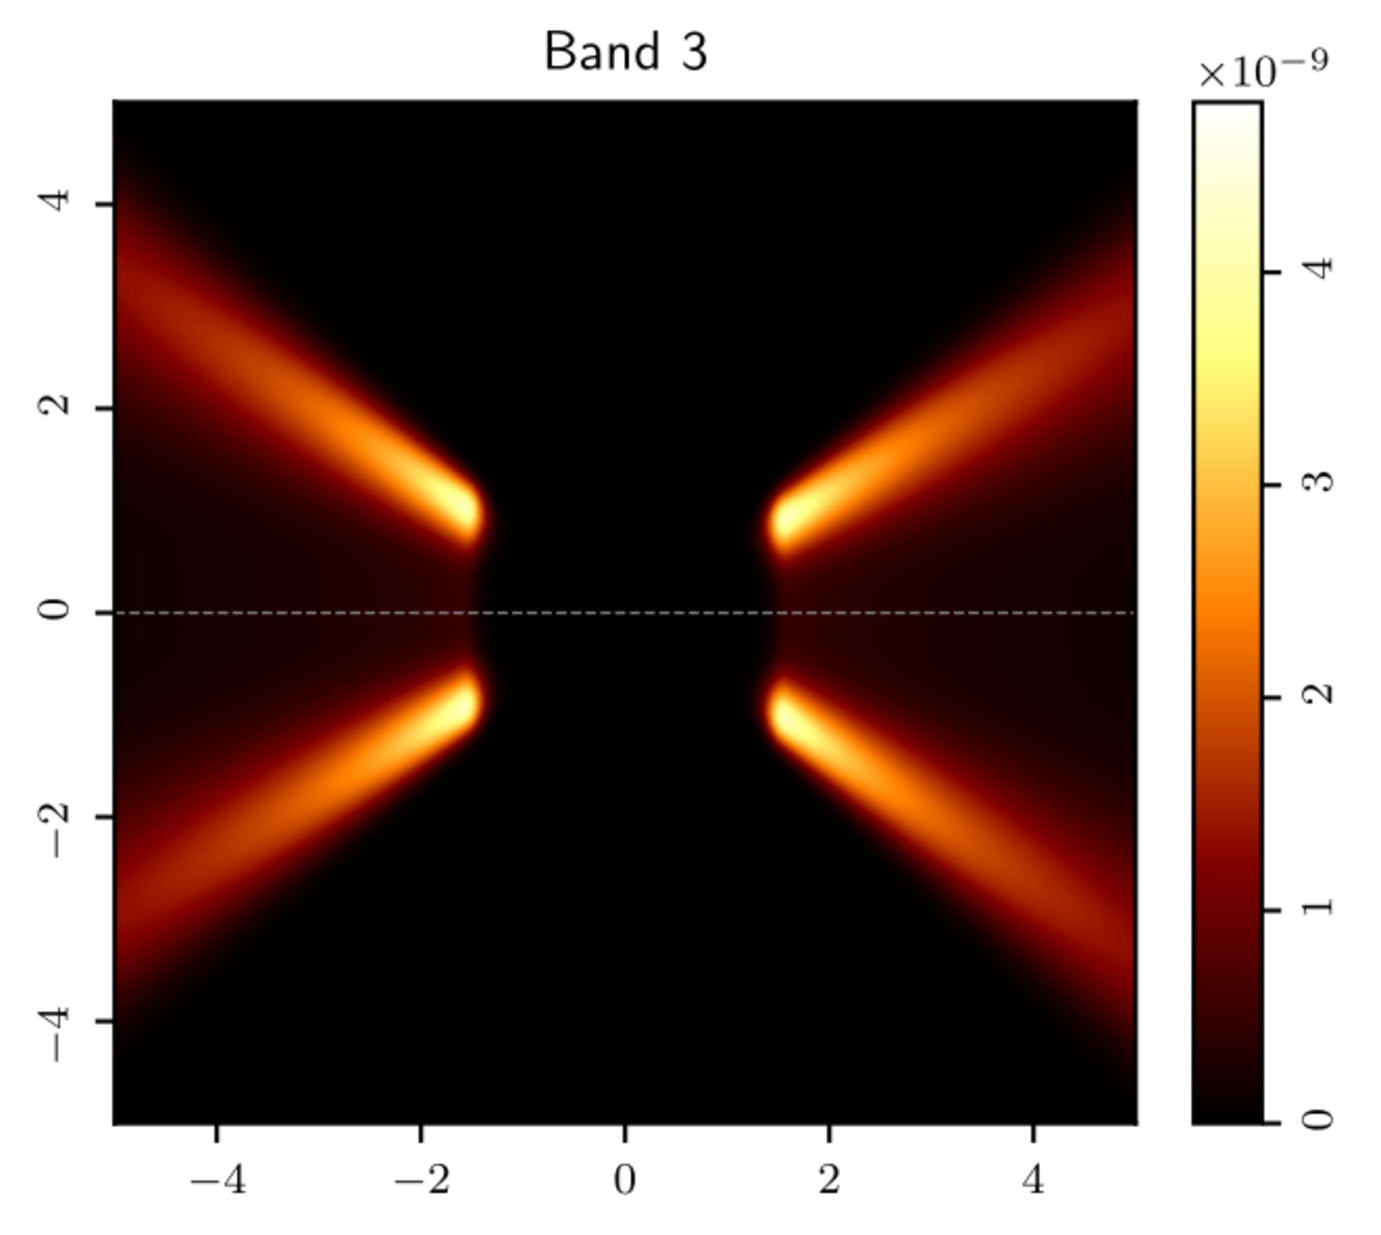
\includegraphics[width=0.95\columnwidth]{figs/band3_cut.pdf}\\
  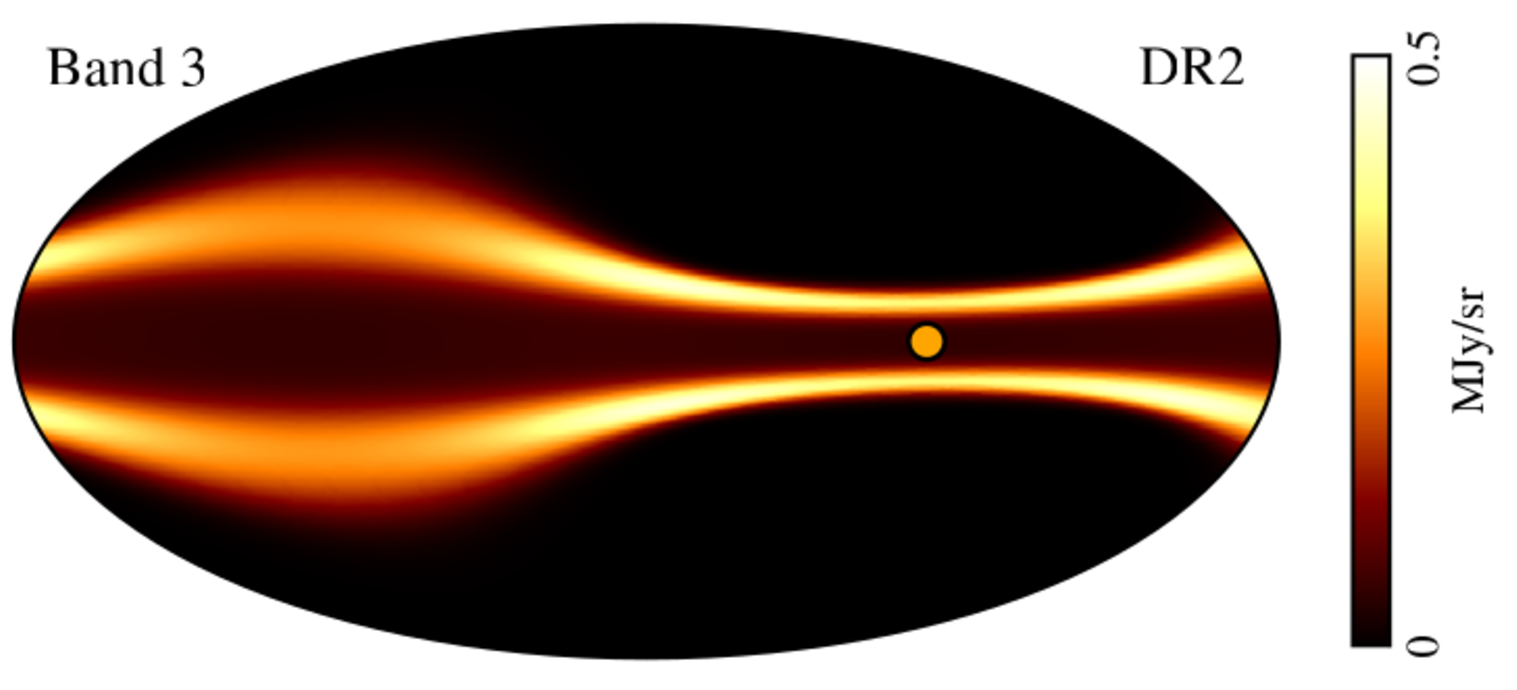
\includegraphics[width=0.95\columnwidth]{figs/band3_instant.pdf}\\
  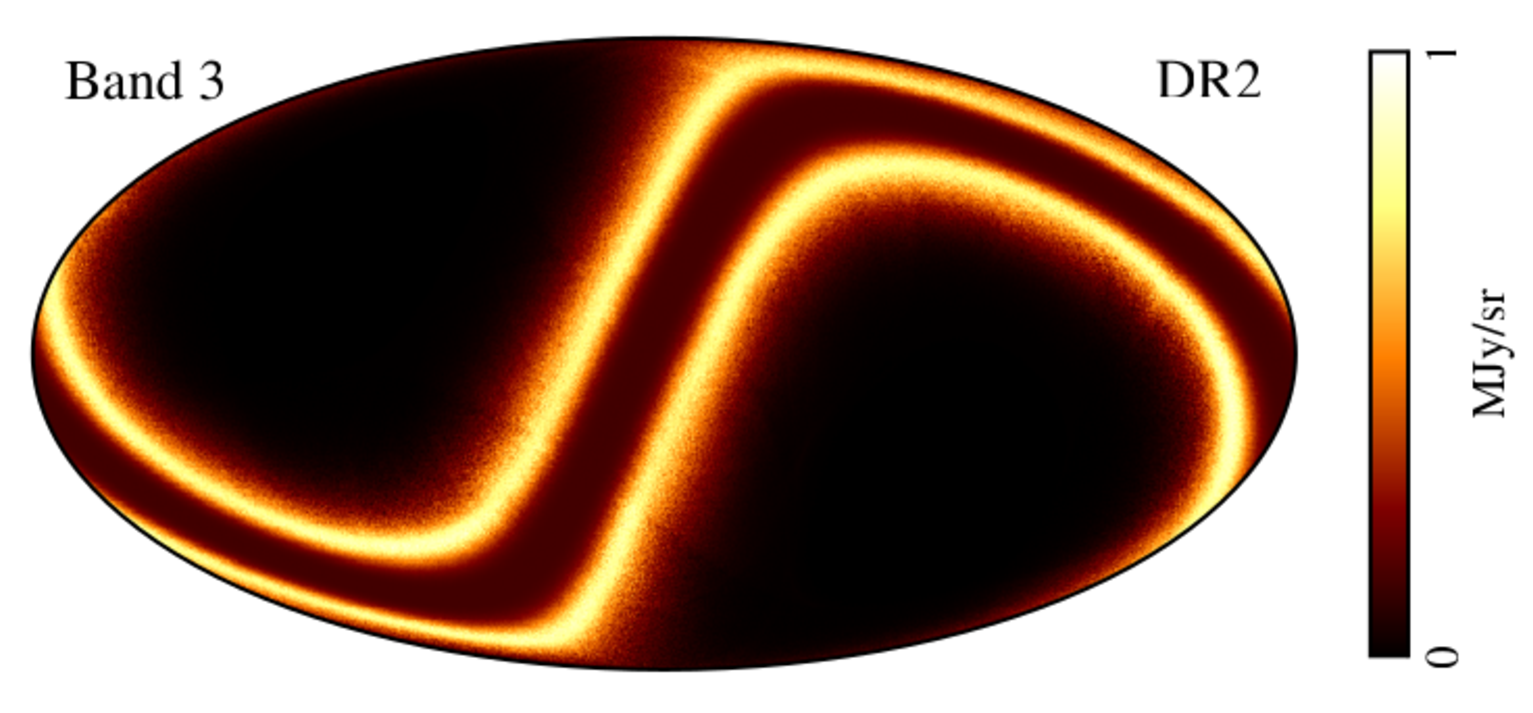
\includegraphics[width=0.95\columnwidth]{figs/band3_mission.pdf}\\
  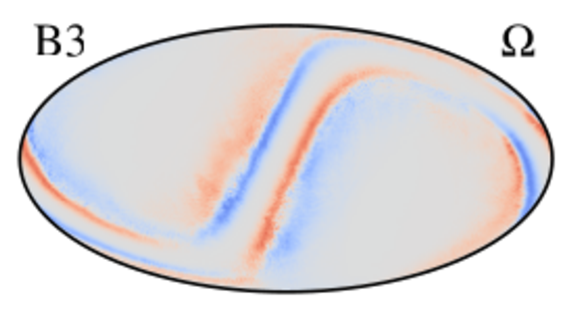
\includegraphics[width=0.95\columnwidth]{figs/band3_omega.pdf}
  \caption{Geometry of the third asteroidal dust band. (\textit{First row}:)
    Slice through the $x$--$z$ plane of the number density, $n_{0}$,
    in heliocentric coordinates. The positions of the Sun and Earth
    are marked by orange and green dots, respectively. (\textit{Second
    panel}:) Observed instantaneous intensity plotted in Ecliptic
    coordinates, obtained by integrating the above figure along each
    line-of-sight. (\textit{Third row}:) Same as above, but plotted in
  Galactic coordinates and averaged over a full year of
  observations. (\textit{Fourth row}:) Difference between observed
  intensities as defined in the third row after changing the value of
  the ascending node, $\Omega$, by 10\,\%. Similar plots for all
  components and parameters are provided in Appendices~\ref{sec:zodi-comps} and \ref{sec:param-atlas}.}
  \label{fig:band3}
\end{figure}

The total intensity from a single IPD grain is then
\begin{align}\label{eq:I_tot}
    I^\mathrm{Total}_{c, \lambda} &= I^\mathrm{Scattering}_{c,\lambda} + I^\mathrm{Thermal}_{c,\lambda}\\
    &= A_{c, \lambda} F_\lambda^\odot \Phi_\lambda + E_{c,\lambda} B_\lambda.
\end{align}
The total ZL signal may then be evaluated by summing up the intensity
from all dust grains, which in practice means evaluating a line-of-sight 
integral for each observation,
\begin{equation}\label{eq:los}
    I_{p,t} = \sum_c \int n_c \left[  A_{c, \lambda} F_\lambda^\odot \Phi_\lambda + \left( 1 - A_{c, \lambda} \right) E_{c,\lambda} B_\lambda \right]\,ds.
\end{equation}
Here, $p$ represents an observed pixel or direction in the sky, $t$ is
the time of observation; $n_c$ is the number density of component $c$
in the line-of-sight; and $ds$ is a small distance along the
line-of-sight $s$ from the observer and towards $p$. Note that
Eqs.~\eqref{eq:los} and~\eqref{eq:I_tot} differ by a factor (1 -
$A_{c, \lambda}$). This factor represents the extinction that occurs
when thermal emission is scattered away from the line-of-sight.

\subsection{Model intuition}

As described above, the K98 model has only $\mathcal{O}(10^2)$ free
parameters. Clearly, this is in reality far too few to fully capture
the true complex nature of ZL across many decades in
wavelength. However, even with such a limited number of parameters,
the model is still severely under-constrained when fitted to the DIRBE
data, and the corresponding posterior distribution exhibits many
strong degeneracies. Consequently, most currently available parameter
estimation algorithms are prone to getting trapped in local posterior
maxima, and this then will result in significant residuals in the
final ZL cleaned maps.

In order to interpret such residuals, and potentially define better
starting points for the non-linear optimization algorithm, it is
useful to build up human visual intuition regarding the impact of each
free parameter. Figure~\ref{fig:band3} shows one specific (and
arbitrary) example of this. First, the top panel shows a
$x$--$z$-plane slice through the three-dimensional IPD number density
distribution for the third dust band, $B_3$. In this figure, the
orange dot markes the Sun's position, while the green dot markes the
observer's (or Earth's) position. Here it is worth noting that this
component is azimuthally symmetric about the Sun, and the full 3D
structure may therefore be visualized by rotating this figure about
the vertical $z$-axis. In this space, it is quite straightforward to
visualize the effect of each free parameter defined by
Eq.~\eqref{eq:band}. For instance, the position of the inner radial
cut-off can be changed by modifying $\delta_{r}$, while the angle
between the $x$-axis and the peak densities may be changed through
$\delta_{\zeta}$. If we modify the $x_0$ offset, the entire density
field will shift left or right.

The second panel in Fig.~\ref{fig:band3} shows the corresponding
signal in Ecliptic coordinates at one single point in time after
integrating the density field along each line-of-sight. The Sun's
position is again marked by an orange dot, but in this case there is
obviously no observer position, since this figure shows the sky as
seen outwards from the observer. In this project 2D space, the
observed structures appear significantly more difficult to visualize
than in 3D space. For instance, while the density of the dust bands
appear symmetric in 3D space, their apparent separation and width as
seen from Earth vary significantly with Ecliptic longitude; they
appear broader in directions that are closer to the Earth, and
narrower where they are further away.

The third panel shows the same feature, but now averaged over a whole
year of observations and plotted in Galactic coordinates. This
represents the signal seen in full-mission maps derived from
DIRBE. Since the underlying IPD structure is azimuthally symmetric
about the Sun, the Earth's movement throughout the year also
symmetrizes the total co-added signal, and the dust bands once again
again symmetric about the Ecliptic plane. However, some small-scale
structures also appear because of small variations in the effective
scanning path of the instrument from day to day; if an entire day's
worth of observations were missing, for instance due to a period of
excessive cosmic ray radiation, strong stripes would appear in this
map.

With the infrastructure for computing such full-mission maps ready at
hand, we can study the impact of each free parameter in greater
detail. As a specific example of this, the bottom panel in
Fig.~\ref{fig:band3} shows the difference between the total signal
obtained when changing the ascending node for Band~3 by 10\,\%
relative to the base model. Intuitively, this corresponds to rotating
the signal in the top figure slightly about the origin. Some parts of
the bands will then appear closer to the Earth, while others will
appear further away. Those regions then in turn appear either red or
blue in the bottom figure. The resulting pattern is a unique
signature for $\Omega$, and if similar structures are observed in the
final ZL cleaned maps, then one should consider modifying this
particular parameter in a future analysis.

Similar figures are provided for all components and all parameters in
Appendices~\ref{sec:zodi-comps} and \ref{sec:param-atlas}, and these
are very useful for building up visual intuition regarding the K98
model. Quickly scanning through the individual panels in
Figs.~\ref{fig:atlas1} and \ref{fig:atlas2}, we can already now
identify strong degeneracies that are likely to turn out problematic
later. For instance, we see that $n_{0,\mathrm{C}}$,
$\alpha_\mathrm{C}$, $n_{0,\mathrm{SR}}$, $T_0$, and $\delta$ are all
dominated by a ring centered along the Ecliptic plane, and these are
likely to interplay significantly. Furthermore, many of these
parameters will obviously also couple significantly to a wide range of
non-ZL type parameters when integrated into a global analysis
framework, including the all-important CIB monopoles, such as
$n_{0,\mathrm{C}}$, $\sigma_{z,\mathrm{SR}}$, and
$\sigma_{\theta,\mathrm{TF}}$.

\begin{figure}
    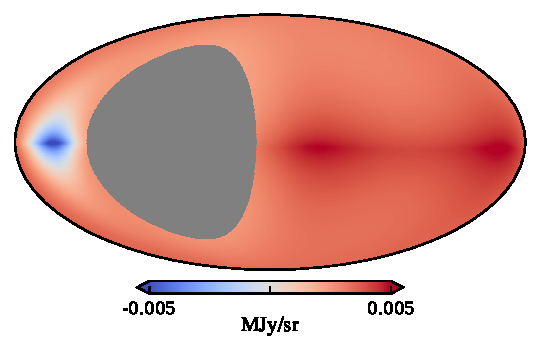
\includegraphics[width=\columnwidth]{figs/cache_error_delta_t.pdf}
    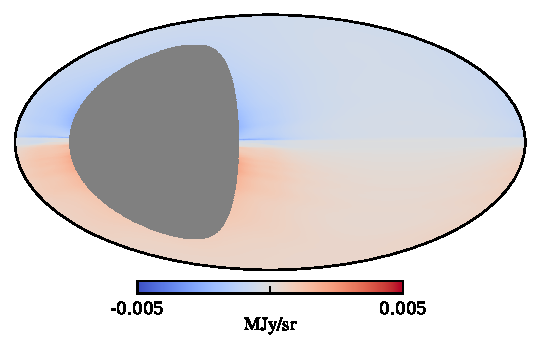
\includegraphics[width=\columnwidth]{figs/cache_error_z.pdf}
    \caption{Errors induced by the ZL cache. \textit{(Top):} Difference between two 
    instantaneous view of the ZL 900\,km above Earth's north and south 
    poles. \textit{(Bottom):} Difference between two instantaneous views of the ZL at $N_\mathrm{studies}=512$, 
    separated by 2 hours. Pixels with an angular separation $\leq 60^\circ$ from the Sun 
    are masked in both maps.}
    \label{fig:cache-error}
\end{figure}



\subsection{Numerical optimizations}\label{sect:optimization}
Performing the line-of-sight integrals defined by Eq.~\eqref{eq:los}
is an expensive part in the \cosmoglobe\ DR2 analysis pipeline already
for the DIRBE data, which only comprise 18\,GB after compression. In
principle, this could be done by brute-force for this particular
experiment on modern computer clusters, but such a direct approach
will clearly not be an option for similar analyses of \Planck\ HFI,
AKARI and SPHEREx. Fortunately, several optimizations are available
for signals that are smooth in both space and time that result in
significant speed-ups at a very low accuracy penalty.

The first and perhaps most trivial optimization is to utilize a ZL
cache coupled to a discrete pixelization. As described in
Sect.~\ref{sect:data}, we employ a HEALPix pixelization with
$7\arcm\times7\arcm$ ($N_{\mathrm{side}}=512$; \citealp{healpix}) in
the current analysis, and all satellite pointings are discretized to
this resolution; that is, we do not account for sub-pixel structure in
the signal model. The cache takes advantage of this by reusing a
previously computed ZL estimate for a given sky pixel when
re-observing a HEALPix pixel within a small timeframe $\Delta t$
\begin{equation}
 s_\mathrm{zodi}(p, t_i) = s_\mathrm{zodi}(p, t_j).
\end{equation}
This cache induces an error on the ZL estimate proportional to $\Delta
t$, which comes from the changes to the observer position with respect
to the zodiacal cloud within the $\Delta t$ timeframe. For reference,
the structure of the ZL on the Ecliptic or Galactic sky maps moves by
about $1^\circ$ a day as the Earth orbits the Sun. The top panel in
Fig.~\ref{fig:cache-error} shows the difference between the exact
instantanous calculation and one that is delayed by $\Delta t =
2\,$hrs for the DIRBE 25\,${\mu}$m channel. The error is less than
1\,kJy/sr, which is more than two orders of magnitude lower than the
total ZL uncertainties. On average, caching reduces the total number
of ZL model evaluations by a factor of $X$.

In addition to the positional change along Earth's orbit, it is
important to note that COBE also orbits the Earth at an altitude of
900\,km. The specific position of the observer is not taken into
account when using the cache. The bottom panel in
Fig.~\ref{fig:cache-error} shows the difference between two
instantaneous full-sky views at 25 $\mu$m, one simulated from the
North pole and the other from the South pole. The magnitude of this
error is $\lesssim\,5$kJy/sr, which is still far below DIRBE's
sensitivity.


The smooth nature of the ZL can be exploited in more ways. When
sampling parameters for the ZL model it is possible to include only a
small fraction of the full dataset in each likelihood evaluation,
simply because the signal-to-noise ratio of each sample is so high,
and because the of the smooth ZL gradient of the ZL
structure. Intuitively speaking, white instrumental noise is
irrelevant compared to overall systematic model uncertainties, and
some number of consecutive time-domain samples therefore provide
essentially the precisely same information. In our current analysis,
we adopt a thinning factor of eight, meaning that we effectively fit
the data to a timestream sampled at 1\,Hz rather than original the
8\,Hz DIRBE CIOs. In principle, we could have averaged over this time
segment, rather than simply omitting the relevant samples, in order to
suppress instrumental noise; and, in fact, the first implementation of
our computer code did exactly this. However, averaging over 1\,sec
time scales implies that the true underlying model is also smoothed
out the same time scales, and this increases the overall modeling
errors. Although the differences were generally small, we obtained
slightly better fits by thinning rather than averaging.

In addition, the smoothness of the ZL is exploited further during
parameter estimation by defining the cache at a pixel resolution of
$1^{\circ}$ ($N_\mathrm{side} = 64$), rather than the original
$N_\mathrm{side} = 512$. We find that this results in very similar
$\chi^2$ values, while further reducing the number of ZL evaluations
used in the sampling steps by a factor of 64. 

\begin{figure*}
    \centering
    \resizebox{\textwidth}{!}{%
    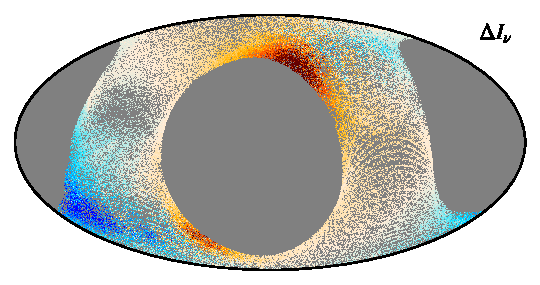
\includegraphics[height=1cm]{figs/week/week_delta_I_nu.pdf}%
    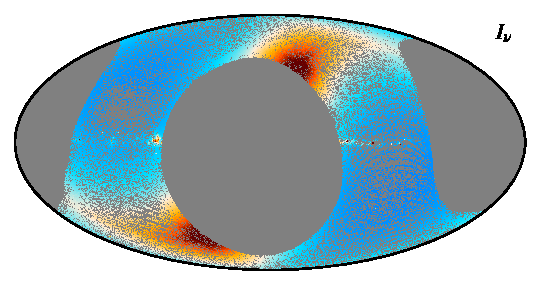
\includegraphics[height=1cm]{figs/week/week_I_nu.pdf}%
    }\\
    \resizebox{\textwidth}{!}{%
    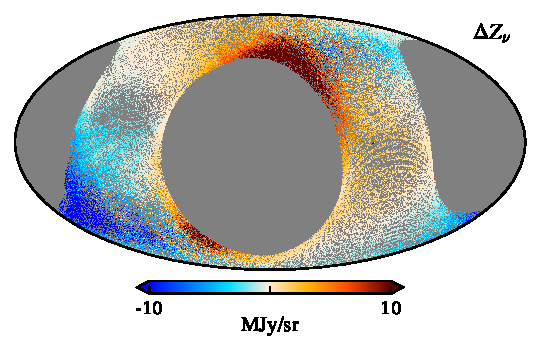
\includegraphics[height=1cm]{figs/week/week_delta_Z_nu.pdf}%
    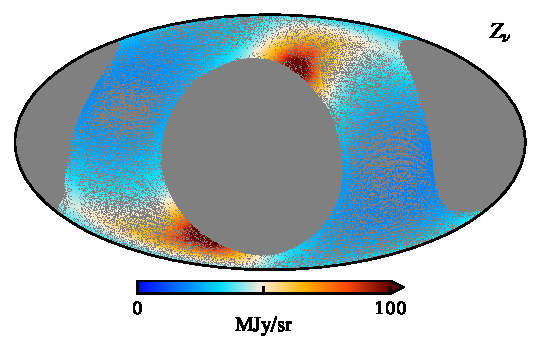
\includegraphics[height=1cm]{figs/week/week_Z_nu.pdf}%
    }\\
    \resizebox{\textwidth}{!}{%
    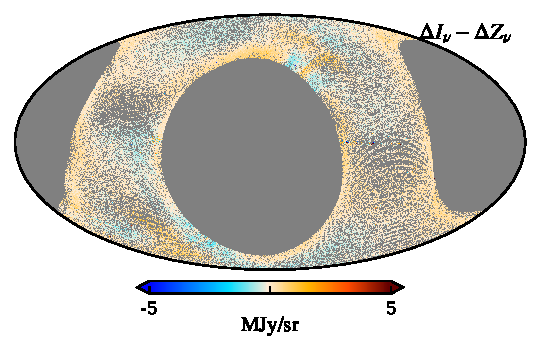
\includegraphics[height=1cm]{figs/week/week_delta_tod_nu.pdf}%
    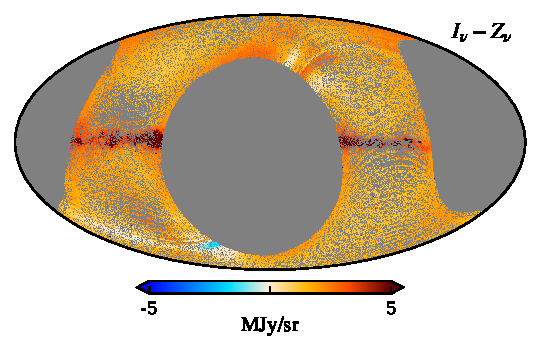
\includegraphics[height=1cm]{figs/week/week_tod_nu.pdf}%
    }\\
    \caption{Illustration of the basic sky maps involved in the zodiacal 
    light fitting algorithms adopted by the DIRBE (\emph{left column}) 
    and \Cosmoglobe\ (\emph{right column}) pipelines for one week of 
    $25\,\mu\mathrm{m}$ observations and adopting the K98 model. The 
    DIRBE pipeline used exclusively differences between weekly and 
    full-season maps, both for the observed signal, 
    $\Delta I_{\nu} \equiv I_{\nu}-\left<I_{\nu}\right>$ (\emph{top left}), 
    and the zodiacal light model, 
    $\Delta Z_{\nu} = Z_{\nu}-\left<Z_{\nu}\right>$ (\emph{middle left}), 
    where brackets indicate full-survey averages. Correspondingly, the 
    final $\chi^2$ is defined through $\Delta I_{\nu} - \Delta Z_{\nu}$ 
    (\emph{bottom left}), and is by constrution only sensitive to 
    time-variable signals. In contrast, the basic data element in 
    \Cosmoglobe\ is the full sky signal, $I_{\nu}$ (\emph{top right}), 
    which is fitted with the full zodiacal light model, $Z_{\nu}$ 
    (\emph{middle right}), both modelled in time-domain. The $\chi^2$ 
    the minimizes minimize the total signal-minus-model residual, 
    $I_{\nu}-Z_{\nu}$ (\emph{bottom right}). The main advantage of the 
    DIRBE approach is insensitivity to stationary sky signals, in 
    particular thermal dust and CIB, while the main advantage of the 
    \Cosmoglobe\ approach is a much higher effective signal-to-noise 
    ratio, both to zodiacal light parameters and zero-levels.}
    \label{fig:week_vs_full}
\end{figure*}


\begin{figure}
    \centering
    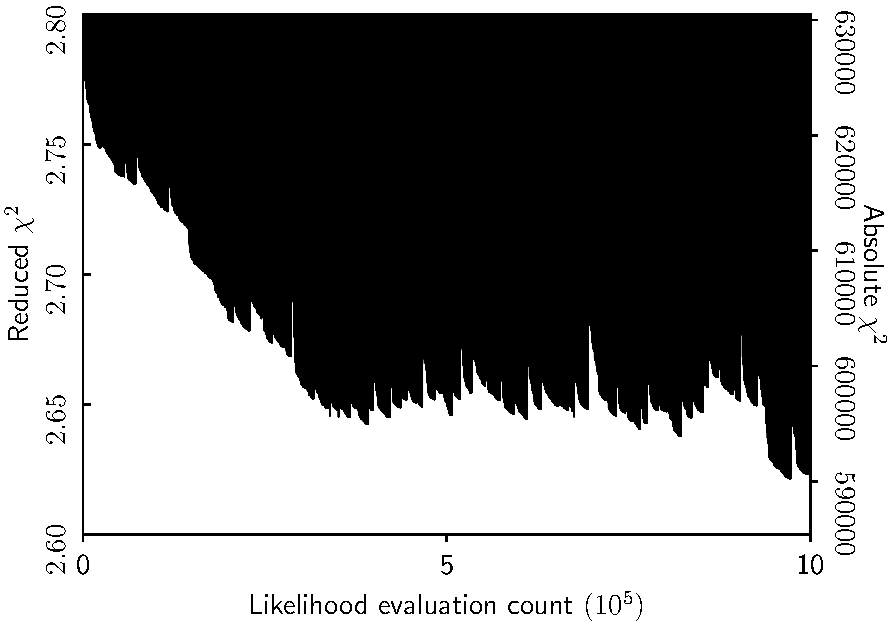
\includegraphics[width=\linewidth]{figs/powell_red_chisq_vs_iter.pdf}
    \caption{Reduced $\chi^2$ as a function of Powell likelihood evaluation count for one single Gibbs chain. Each discrete jump indicates the start of a new Gibbs sample, which is initialized on a new random point that is close to the previous iteration. The following systematic decline within each main Gibbs iteration indicates the non-linear optimization performed by the Powell algorithm.  The solid dark region corresponds to a large number of highly sub-optimal parameter trials. }
    \label{fig:powell_chisq_iter}
\end{figure}


\begin{figure}
    \centering
    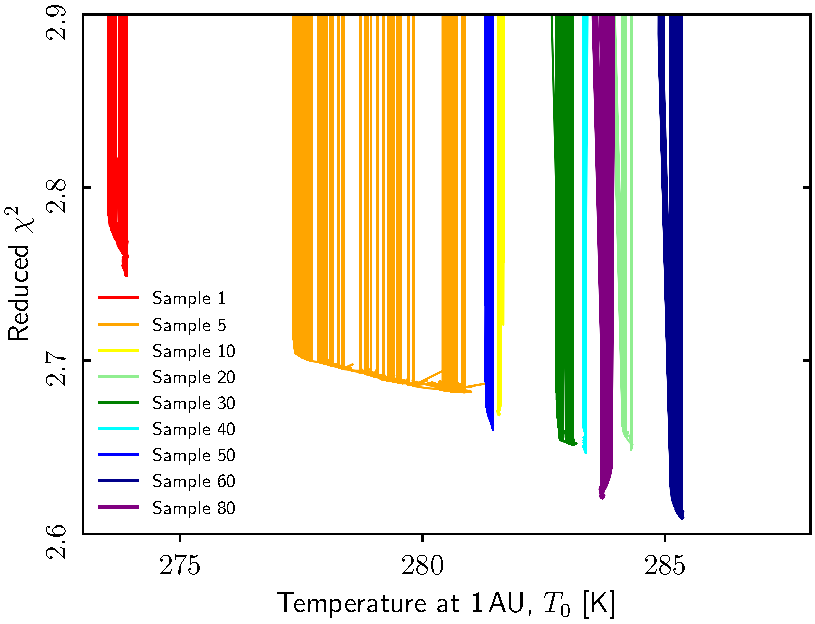
\includegraphics[width=\linewidth]{figs/powell_T0_vs_chisq.pdf}
    \caption{Reduced $\chi^2$ as a function of the temperature at 1\,AU, $T_0$. Each curve shows the full set of parameter trials within one single main Gibbs iteration (or Powell call), and different colors indicate different Gibbs iteration. Redder colors are earlier in the chain.}
    \label{fig:powell_T0}
\end{figure}


\section{Data}\label{sect:data}

\subsection{DIRBE Calibrated Individual Observations}

\subsection{Masks}


\begin{figure}
    \centering
    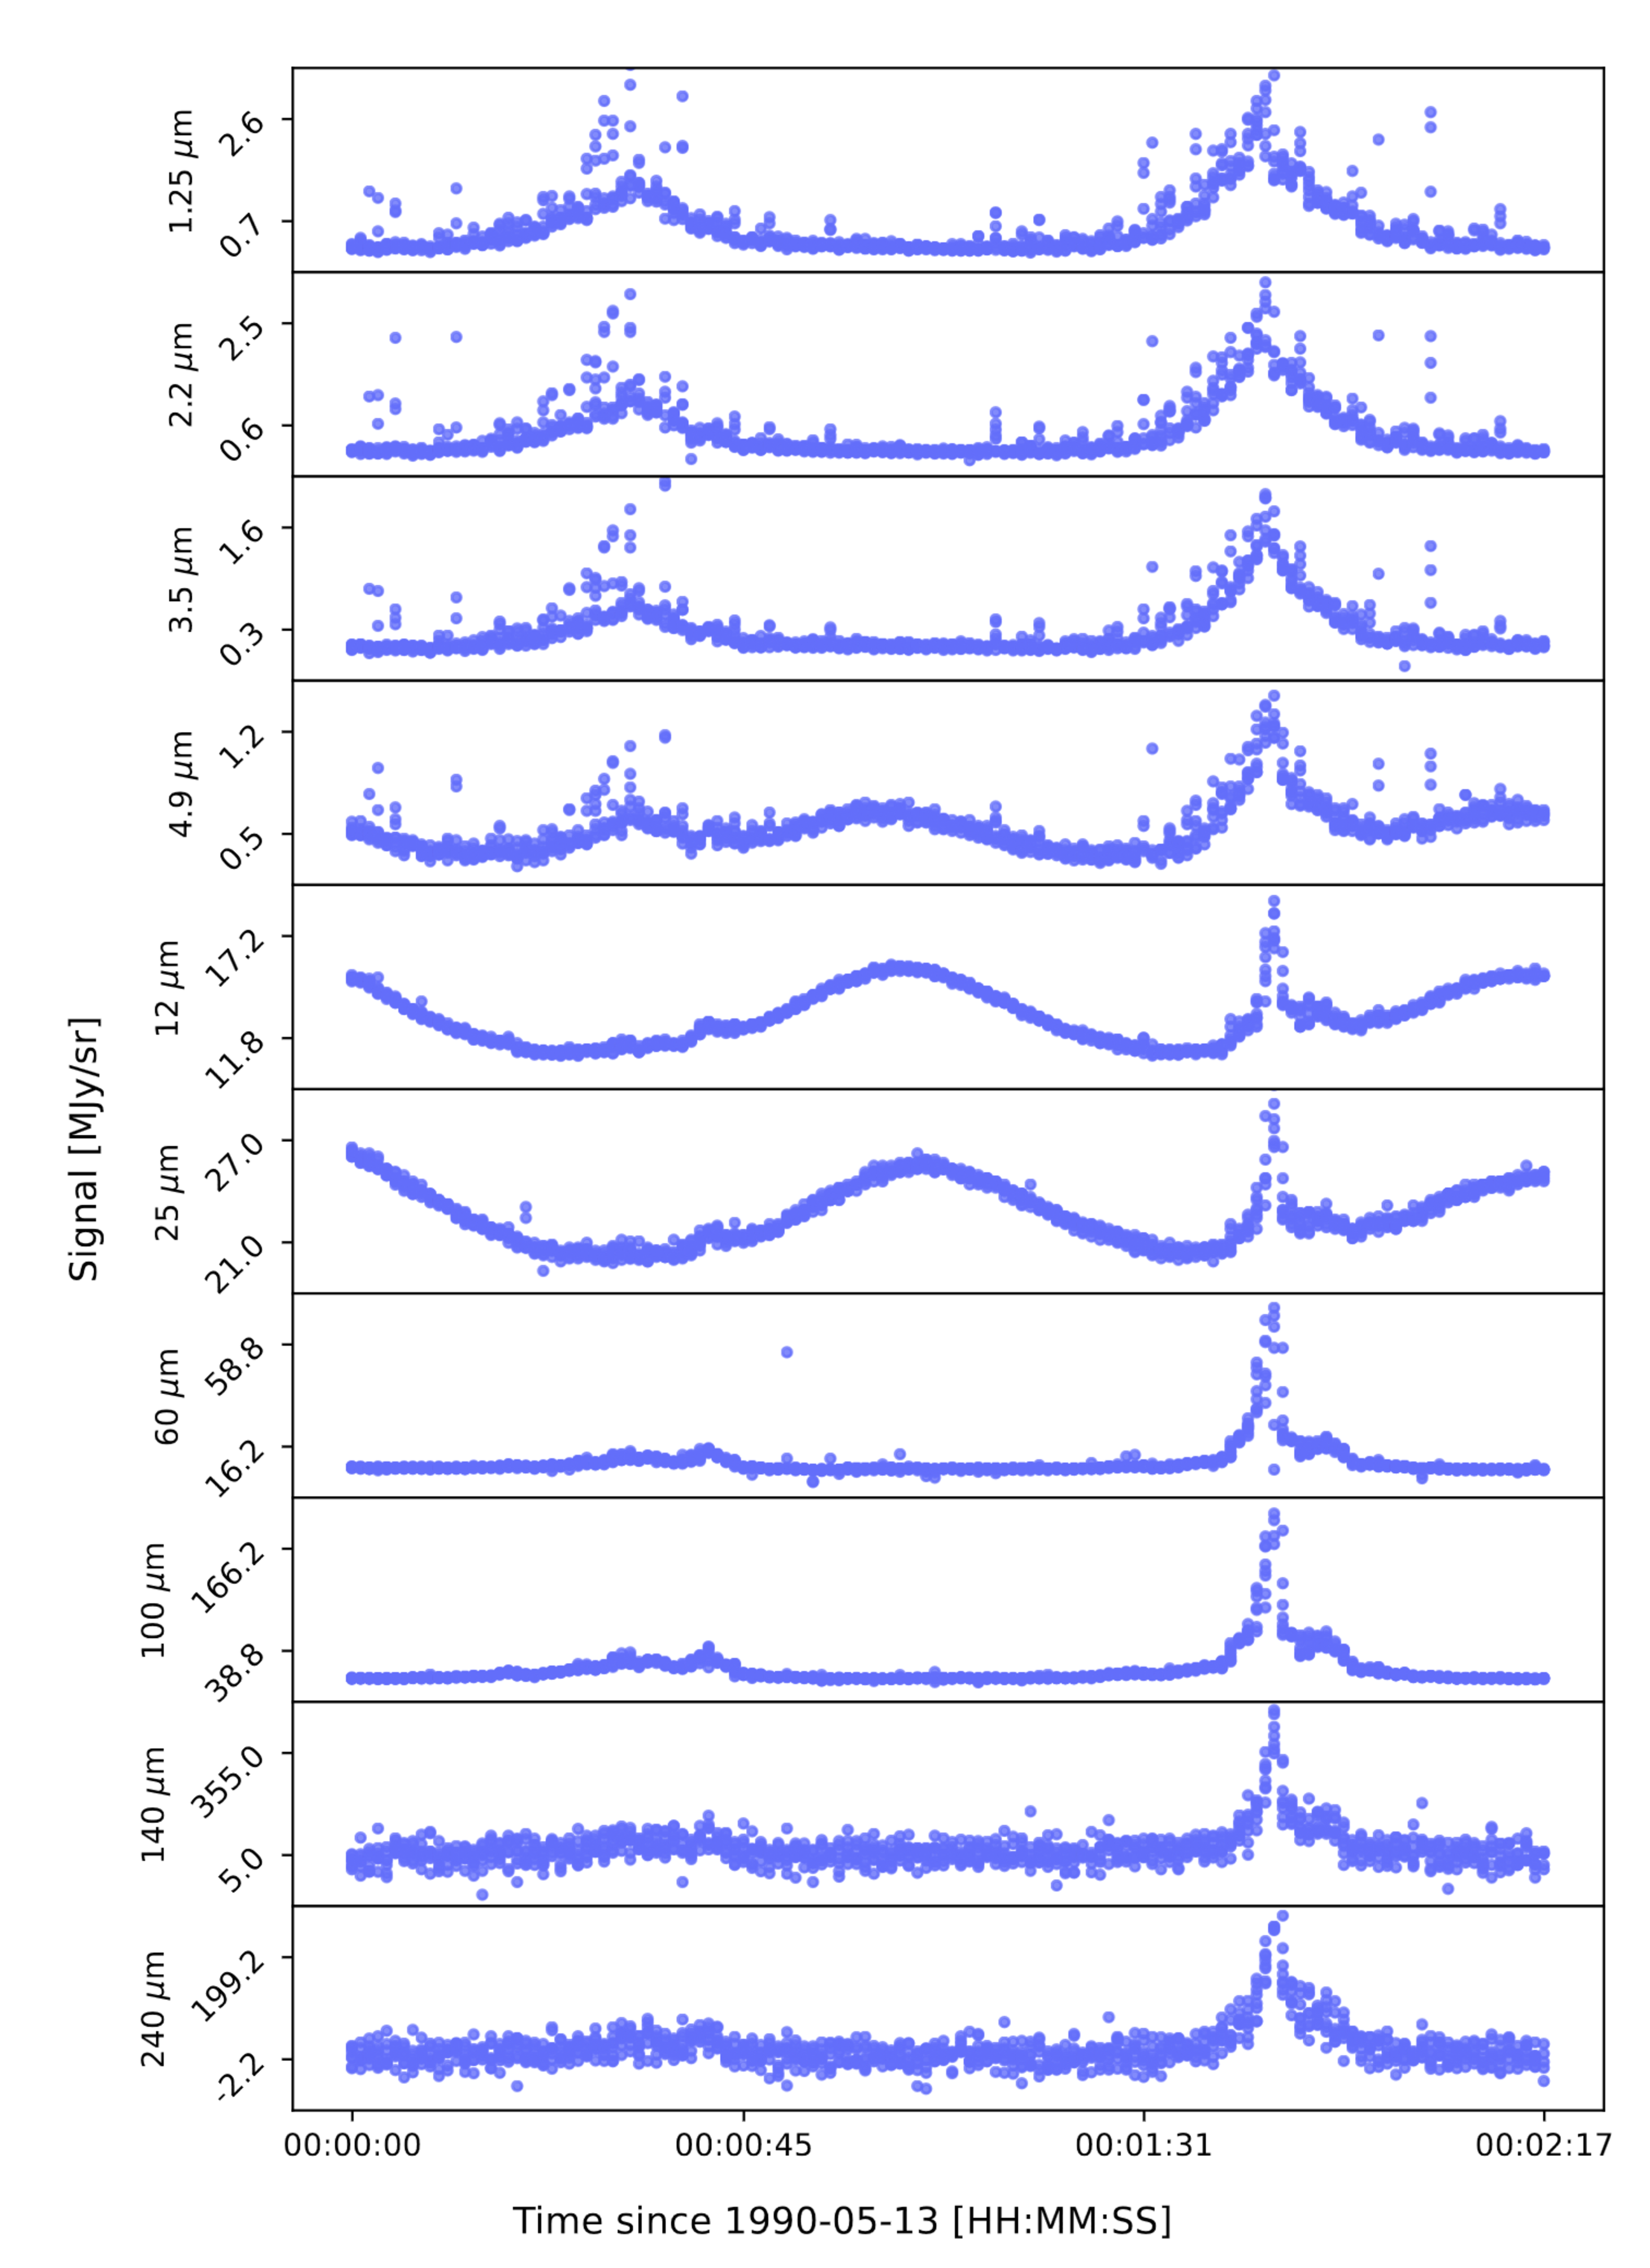
\includegraphics[width=\columnwidth]{figs/tod_zodi.pdf}
    \caption{}
    \label{fig:tod_zodi}
\end{figure}


\begin{figure}
    \centering
    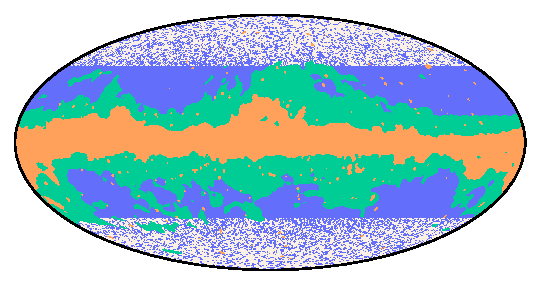
\includegraphics[width=\columnwidth]{figs/zodi_proc_masks.pdf}
    \caption{Three of the processing masks used when estimating ZL parameters. The blue mask is the 
    mask used in the stellar emission dominated 1.25 $\mathrm{\mu m}$ band, the orange mask is used 
    in the ZL dominated 25 $\mathrm{\mu m}$ band, and the green mask is used in the thermal dust dominated 
    240 $\mathrm{\mu m}$ band.}
    \label{fig:zodi-procmask}
\end{figure}





\section{Methods}\label{sect:param-estimation}

\subsection{Bayesian analysis, posterior distribution, and Gibbs sampling}

Estimating the ZL model parameters happens within the Bayesian end-to-end Commander3 framework. An explaination of the algorithms used to fit the full data and sky model, as well as instrumental parameters are described in detail in \cite{CG02_01}. In short, we use Gibbs sampling to map out the joint posterior distribution\citep{Galloway2023}, which allows us to draw samples iteratively from various conditional distributions rather than trying to draw directly from a large and complicated joint distribution. The following equations show each parameter sampled in this Cosmoglobe analysis in order
\begin{alignat}{11}
    \tens{G} &\,\leftarrow P(\tens{G}&\,\mid &\,\dv,&\, &\,\phantom{\tens{G}} &\,\xi_n, &
    \,\beta_{\mathrm{sky}}& \,\a_{\mathrm{sky}}, &\,\zeta_{\mathrm{z}},
    &\,\a_{\mathrm{static}})\label{eq:gibbs_G}\\
    \xi_{\mathrm{n}} &\,\leftarrow P(\xi_{\mathrm{n}}&\,\mid &\,\dv,&\, &\,\tens{G}, &\,\phantom{\xi_n} &
    \,\beta_{\mathrm{sky}}& \,\a_{\mathrm{sky}}, &\,\zeta_{\mathrm{z}},
    &\,\a_{\mathrm{static}})\\
    \beta_{\mathrm{sky}} &\,\leftarrow P(\beta_{\mathrm{sky}}&\,\mid &\,\dv,&\, &\,\tens{G}, &\,\xi_n, &
    \,\phantom{\beta_{\mathrm{sky}}}& \,\a_{\mathrm{sky}}, &\,\zeta_{\mathrm{z}}, &\,\a_{\mathrm{static}})\\
    \a_{\mathrm{sky}} &\,\leftarrow P(\a_{\mathrm{sky}}&\,\mid &\,\dv,&\, &\,\tens{G}, &\,\xi_n, &
    \,\beta_{\mathrm{sky}},& \,\phantom{\a_{\mathrm{sky}},}
    &\,\zeta_{\mathrm{z}}, &\,\a_{\mathrm{static}})\\
    \zeta_{\mathrm{z}} &\,\leftarrow P(\zeta_{\mathrm{z}}&\,\mid &\,\dv,&\, &\,\tens{G}, &\,\xi_n, &
    \,\beta_{\mathrm{sky}},& \,\a_{\mathrm{sky}},
    &\,\phantom{\zeta_{\mathrm{z}},} &\,\a_{\mathrm{static}})\label{eq:gibbs_zodi}\\
    \a_{\mathrm{static}} &\,\leftarrow P(\a_{\mathrm{static}}&\,\mid &\,\dv,&\, &\,\tens{G}, &\,\xi_n, &
    \,\beta_{\mathrm{sky}},& \,\a_{\mathrm{sky}}, &\,\zeta_{\mathrm{z}} &\,\phantom{\a_{\mathrm{static}}})\label{eq:gibbs_static}.
\end{alignat}
Each of the sampling steps in the above Gibbs chain is described by \citet{CG02_01}
and references therin. 

For computational reasons it is sometimes necessary to violate the Gibbs rule,
which is the case for the step in Equation~\ref{eq:gibbs_zodi}, which describes
the sampling of the ZL parameters, denoted by $\zeta_\mathrm{z}$. The K98 ZL 
model contains around 50 parameters to describe the three-dimensional IPD 
distribution and another 30 or more to describe the thermal emission and 
scattered sunlight source functions, many of which are heavily degenerate
due to the difficulties of mapping a three-dimensional structure from a single
data set. N of these parameters were fit to the DIRBE data, in the original DIRBE analysis while the rest were fixed to parameters motivated by studies of the interplanetary medium. In our analysis we have fit M total parameters. A visualization of the degeneracies and the way in which each ZL parameter impacts the final mission-averaged predicted ZL are seen in figures~\ref{fig:atlas1} and~\ref{fig:atlas2} in Appendix~\ref{sec:param-atlas}. This atlas of ZL parameters shows normalized maps of the effects of changing a single ZL parameter by $\pm 5\%$ while keeping the rest of the model fixed. The albedo and emissivity parameters are excluded from the atlas as these represent a direct scaling of the component maps and are degenerate with the $n_0$ maps.
The posterior distribution of this complicated set of parameters exhibits a large number of local minima due to the above mentioned reasons. When experimenting we found that strict Gibbs sampling algorithm quickly became trapped. We have opted to instead 
use a simple non-linear Powell algorithm that is initialized some random parameter distance away from the previous sample, and then searches for the local minimum. Powell's method is a function minimizer, which performs bi-directional searches along a parameter vector. This algorithm is able to escape local minima, but it comes at the cost of larger
uncertainties than what would result from an ideal posterior mapper.


The K98 model was obtained by fitting the model to a set of week-maps. 
The $\chi^2$ measure used by the DIRBE team is given by
\begin{equation}
    \chi^2_\mathrm{K98} = \Delta I_\nu - \Delta Z_\nu,
\end{equation}
where $I_\nu$ and $Z_\nu$ are the full-mission frequency and ZL estimate 
maps, and $\Delta I_\nu = I_\nu - \langle I_\nu \rangle$ and $\Delta Z_\nu = Z_\nu - \langle Z_\nu \rangle$ are the difference between 
the full-mission and a week frequency and ZL map, respectively. These 
maps are illustrated in the left column in Figure~\ref{fig:week_vs_full}. 
$\chi^2_\mathrm{K98}$ is by construction only sensitive to time-variable 
signal, effectively removing the need for a good sky model of the then 
less well-understood infrared sky. Using week maps instead of the full 
timestreams has the additional effect of reducing the overall data 
volume in the fits, which would seem beneficial considering the 
computing resources available during the early DIRBE analysis. A 
downside of this method is that the monopole induced by the smooth ZL is 
removed, resulting in a much weaker signal-to-noise ratio in the ZL 
parameter estimates and to the zero-levels. In contrast, we fit the data 
at each time step to the signal minus model residual
\begin{equation}\label{eq:chisq}
    \chi^2 = I_\nu - Z_\nu.
\end{equation}
To minimize the amount of unmodeled galactic emission that enters our 
ZL parameter estimates, we use strict channel-specific processing masks, 
masking out the brightest galactic regions. The 1.25, 25, and 240 $\mu$m 
masks, corresponding to stellar light, ZL, and thermal dust-dominated 
channels, are shown in Figure~\ref{fig:zodi-procmask}.


\subsection{Non-linear posterior maximization}

The total number of free ZL model parameters in this analysis are N, 
compared to the M parameters fit in K98. We have included a non-zero
scattering contribution at 4.9 $\mu$m. The ZL SED is composition of two
blackbody like spectra with a combined minimum around the $3.5\mu$m band. The first
blackbody spectrum is associated with the solar flux through the scattering 
contribution, while the second with the re-radiated thermal emission. With an
improved sky model and lower residual levels, we believe that it is worth 
including the small non-zero contribution from scattering at 4.9 $\mu$m.
Additionally, we are using the 12 $\mu$m band as our ZL reference band, meaning
that we fix the emissivities at this band to 1 \textcolor{red}{(why?)}. The
reference ZL band in K98 is $25 \mu$m. Similar to K98, we fit one emissivity 
for the smooth cloud, and one joint emissivity for the dust bands, while we 
only fit one overall albedo for all components, at each frequency band. Where,
K98 fixed emissivities to the cloud at certian bands, we have kept all free.

We can improve our error estimates on the ZL parameters by including the 
Powell search history in our error estimation. For each bi-directional 
search, we output both the parameter values and the intermediate $\chi^2$
values which lets us find the 95\% confidence interval in the search. This
is used jointly with the uncertienties determined from the Gibbs chain.
\textcolor{red}{Do this with Duncan}

\subsection{Computational costs and optimization}


\section{Results}\label{sect:improved-model}
Here we present our best-fit ZL model from having run Commander3 for six independant
Markov Chains for N samples. Our best-fit parameters for the geometrical IPD, emissivities 
and albedo parameters are listed in tables~\ref{table:zodi-params-geo} 
and~\ref{table:zodi-params-spectral}, where they are compared to the values in the K98 model.


\begin{table*}
    \small
    \centering
    \newcolumntype{C}{ @{}>{${}}r<{{}$}@{} }
    \begin{tabular}{l l *2{rCl}}
    \hline
    \hline
     Parameter & Description & \multicolumn{3}{c}{DIRBE} & \multicolumn{3}{c}{Cosmoglobe DR2} \\ 
     \hline
     \multicolumn{8}{c}{Smooth Cloud}\\
     \hline
     $n_{0, \mathrm{C}}$ [$10^{-7}$ AU$^{-1}$] & Number density & 1.13 &\pm& 0.0064 & 1.13 &\pm& 0.0064\\
     $\alpha$ & Radial power-law exponent \quad& 1.34 &\pm& 0.022 & 1.13 &\pm& 0.0064\\
     $\beta$ & Vertical shape parameter & 4.14 &\pm& 0.067 & 1.13 &\pm& 0.0064\\
     $\gamma$ & Vertical power-law exponent & 0.942 &\pm& 0.025 & 1.13 &\pm& 0.0064\\
     $\mu$ & Widening parameter & 0.189 &\pm& 0.014 & 1.13 &\pm& 0.0064\\
     $i$ [deg] & Inclination & 2.03 &\pm& 0.017 & 1.13 &\pm& 0.0064\\
     $\Omega$ [deg] & Ascending node & 77.7 &\pm& 0.6 & 1.13 &\pm& 0.0064\\
     $X_0$ [$10^{-3}$ AU] & x-offset from the Sun  & 11.9 &\pm& 1.1 & 1.13 &\pm& 0.0064\\
     $Y_0$ [$10^{-3}$ AU] & y-offset from the Sun & 5.48 &\pm& 0.77 & 1.13 &\pm& 0.0064\\
     $Z_0$ [$10^{-3}$ AU] & z-offset from the Sun & -2.15 &\pm& 0.43 & 1.13 &\pm& 0.0064\\
     \hline
     \multicolumn{8}{c}{Dust band 1}\\
     \hline
     $n_{0, \mathrm{B}_1}$ [$10^{-10}$ AU$^{-1}$] & Number density & 5.59 &\pm& 0.72 & 1.13 &\pm& 0.0064\\
     $\delta_{\zeta_{\mathrm{B}_1}}$ [deg] & Shape parameter & 8.78 && Fixed & 1.13 &\pm& 0.0064\\
     $v_{\mathrm{B}_1}$ & Shape parameter & 0.10 && Fixed & 1.13 &\pm& 0.0064\\
     $p_{\mathrm{B}_1}$ & Shape parameter & 4 && Fixed & 0.10 &\pm& 0.0064\\
     $i_{\mathrm{B}_1}$ [deg] & Inclination & 0.56 && Fixed & 0.10 &\pm& 0.0064\\
     $\Omega_{\mathrm{B}_1}$ [deg] & Ascending node & 80 && Fixed & 0.10 &\pm& 0.0064\\
     $\delta_{R_{\mathrm{B}_1}}$ [AU] & Inner radial cutoff & 1.5 && Fixed & 0.10 &\pm& 0.0064\\
     \hline
     \multicolumn{8}{c}{Dust band 2}\\
     \hline
     $n_{0, \mathrm{B}_2}$ [$10^{-9}$ AU$^{-1}$] & Number density & 1.99 &\pm& 0.128 & 1.13 &\pm& 0.0064\\
     $\delta_{\zeta_{\mathrm{B}_2}}$ [deg] & Shape parameter & 1.99 && Fixed & 1.13 &\pm& 0.0064\\
     $v_{\mathrm{B}_2}$ & Shape parameter & 0.9 && Fixed & 1.13 &\pm& 0.0064\\
     $p_{\mathrm{B}_2}$ & Shape parameter & 4 && Fixed & 0.10 &\pm& 0.0064\\
     $i_{\mathrm{B}_2}$ [deg] & Inclination & 1.2 && Fixed & 0.10 &\pm& 0.0064\\
     $\Omega_{\mathrm{B}_2}$ [deg] & Ascending node & 30.3 && Fixed & 0.10 &\pm& 0.0064\\
     $\delta_{R_{\mathrm{B}_2}}$ [AU] & Inner radial cutoff & 0.94 &\pm& 0.025 & 0.10 &\pm& 0.0064\\
     \hline
     \multicolumn{8}{c}{Dust band 3}\\
     \hline
     $n_{0, \mathrm{B}_3}$ [$10^{-10}$ AU$^{-1}$] & Number density & 1.44 &\pm& 0.234 & 1.13 &\pm& 0.0064\\
     $\delta_{\zeta_{\mathrm{B}_3}}$ [deg] & Shape parameter & 15 && Fixed & 1.13 &\pm& 0.0064\\
     $v_{\mathrm{B}_3}$ & Shape parameter & 0.05 && Fixed & 1.13 &\pm& 0.0064\\
     $p_{\mathrm{B}_3}$ & Shape parameter & 4 && Fixed & 0.10 &\pm& 0.0064\\
     $i_{\mathrm{B}_3}$ [deg] & Inclination & 0.8 && Fixed & 0.10 &\pm& 0.0064\\
     $\Omega_{\mathrm{B}_3}$ [deg] & Ascending node & 80 && Fixed & 0.10 &\pm& 0.0064\\
     $\delta_{R_{\mathrm{B}_3}}$ [AU] & Inner radial cutoff & 1.5 && Fixed & 0.10 &\pm& 0.0064\\
     \hline
     \multicolumn{8}{c}{Circum-solar ring}\\
     \hline
     $n_{0, \mathrm{SR}}$ [$10^{-8}$ AU$^{-1}$] & Number density & 1.83 &\pm& 0.127 & 1.13 &\pm& 0.0064\\
     $R_\mathrm{SR}$ [AU] & Radius of peak number density & 1.03 &\pm& 0.00064 & 1.13 &\pm& 0.0064\\
     $\sigma_{r,\mathrm{SR}}$ [AU] & Radial dispersion & 0.025 && Fixed & 1.13 &\pm& 0.0064\\
     $\sigma_{z,\mathrm{SR}}$ [AU] & Vertical dispersion & 0.054 &\pm& 0.0066 & 1.13 &\pm& 0.0064\\
     $i_{\mathrm{SR}}$ [deg] & Inclination & 0.49 &\pm& 0.063 & 0.10 &\pm& 0.0064\\
     $\Omega_{\mathrm{SR}}$ [deg] & Ascending node & 22.3 &\pm& 0.0014 & 0.10 &\pm& 0.0064\\
     \hline
     \multicolumn{8}{c}{Earth-trailing feature}\\
     \hline
     $n_{0, \mathrm{TB}}$ [$10^{-8}$ AU$^{-1}$] & Number density & 1.9 &\pm& 0.142 & 1.13 &\pm& 0.0064\\
     $R_\mathrm{TB}$ [AU] & Radius of peak number density & 1.06 &\pm& 0.011 & 1.13 &\pm& 0.0064\\
     $\sigma_{r,\mathrm{TB}}$ [AU] & Radial dispersion & 0.10 &\pm& 0.0097 & 1.13 &\pm& 0.0064\\
     $\sigma_{z,\mathrm{TB}}$ [AU] & Vertical dispersion & 0.091 &\pm& 0.013 & 1.13 &\pm& 0.0064\\
     $\theta_{\mathrm{TB}}$ [deg] & Longitude with respect to Earth  & -10 && Fixed & 0.10 &\pm& 0.0064\\
     $\sigma_{\theta,\mathrm{TB}}$ [deg] & Longitude dispersion & 12.1 &\pm& 3.4 & 0.10 &\pm& 0.0064\\
     \hline
    \end{tabular}
    \caption{Comparison between best-fit number density and geometrical 
    interplanetary dust parameters in the DIRBE model and our model.}
    \label{table:zodi-params-geo}
    \end{table*}
    
\begin{table*}
    \small
    \centering
    \newcolumntype{C}{ @{}>{${}}r<{{}$}@{} }
    \begin{tabular}{l l *2{rCl}}
    \hline
    \hline
     Parameter & Description & \multicolumn{3}{c}{DIRBE} & \multicolumn{3}{c}{Cosmoglobe DR2} \\ 
     \hline
     \multicolumn{8}{c}{Smooth Cloud}\\
     \hline
     $A_1$ & Albedo at 1.25$\mu $m & 0.204 &\pm& 0.0013 & 1.13 &\pm& 0.0064\\
     $A_2$ & Albedo at 2.2$\mu $m & 0.255 &\pm& 0.0017 & 1.13 &\pm& 0.0064\\
     $A_3$ & Albedo at 3.5$\mu $m & 0.210 &\pm& 0.019 & 1.13 &\pm& 0.0064\\
     $A_4$ & Albedo at 4.9$\mu $m  & 0 && Fixed & 1.13 &\pm& 0.0064\\
     $E_3$ & Emissivity at 3.5$\mu $m  & 1.66 &\pm& 0.088 & 1.13 &\pm& 0.0064\\
     $E_4$ & Emissivity at 4.9$\mu $m  & 0.997 &\pm& 0.0036 & 1.13 &\pm& 0.0064\\
     $E_5$ & Emissivity at 12$\mu $m  & 0.958 &\pm& 0.0026 & 1.13 &\pm& 0.0064\\
     $E_6$ & Emissivity at 25$\mu $m  & 1 && Fixed & 1.13 &\pm& 0.0064\\
     $E_7$ & Emissivity at 60$\mu $m  & 0.733 &\pm& 0.0055 & 1.13 &\pm& 0.0064\\
     $E_8$ & Emissivity at 100$\mu $m  & 0.647 &\pm& 0.012 & 1.13 &\pm& 0.0064\\
     $E_9$ & Emissivity at 140$\mu $m  & 0.677 && ? & 1.13 &\pm& 0.0064\\
     $E_{10}$ & Emissivity at 240$\mu$m    & 0.519 && ? & 1.13 &\pm& 0.0064\\
     \hline
     \multicolumn{8}{c}{Dust bands}\\
     \hline
     \hline
     $A_1$ & Albedo at 1.25$\mu $m & 0.204 && Fixed to smooth cloud & 1.13 &\pm& 0.0064\\
     $A_2$ & Albedo at 2.2$\mu $m & 0.255 && Fixed to smooth cloud & 1.13 &\pm& 0.0064\\
     $A_3$ & Albedo at 3.5$\mu $m & 0.210 && Fixed to smooth cloud & 1.13 &\pm& 0.0064\\
     $A_4$ & Albedo at 4.9$\mu $m  & 0 && Fixed & 1.13 &\pm& 0.0064\\
     $E_3$ & Emissivity at 3.5$\mu $m  & 1.66 && Fixed to smooth cloud & 1.13 &\pm& 0.0064\\
     $E_4$ & Emissivity at 4.9$\mu $m  & 0.359 &\pm& 0.054 & 1.13 &\pm& 0.0064\\
     $E_5$ & Emissivity at 12$\mu $m  & 1.01 &\pm& 0.15 & 1.13 &\pm& 0.0064\\
     $E_6$ & Emissivity at 25$\mu $m  & 1 && Fixed & 1.13 &\pm& 0.0064\\
     $E_7$ & Emissivity at 60$\mu $m  & 1.25 &\pm& 0.3 & 1.13 &\pm& 0.0064\\
     $E_8$ & Emissivity at 100$\mu $m  & 1.52 &\pm& 0.65 & 1.13 &\pm& 0.0064\\
     $E_9$ & Emissivity at 140$\mu $m  & 1.13 && ? & 1.13 &\pm& 0.0064\\
     $E_{10}$ & Emissivity at 240$\mu $m  & 1.40 && ? & 1.13 &\pm& 0.0064\\
     \hline
     \multicolumn{8}{c}{Circum-solar ring and Earth-trailing feature}\\
     \hline
     \hline
     $A_1$ & Albedo at 1.25$\mu $m & 0.204 && Fixed to smooth cloud & 1.13 &\pm& 0.0064\\
     $A_2$ & Albedo at 2.2$\mu $m & 0.255 && Fixed to smooth cloud & 1.13 &\pm& 0.0064\\
     $A_3$ & Albedo at 3.5$\mu $m & 0.210 && Fixed to smooth cloud & 1.13 &\pm& 0.0064\\
     $A_4$ & Albedo at 4.9$\mu $m  & 0 && Fixed & 1.13 &\pm& 0.0064\\
     $E_3$ & Emissivity at 3.5$\mu $m  & 1.66 && Fixed to smooth cloud & 1.13 &\pm& 0.0064\\
     $E_4$ & Emissivity at 4.9$\mu $m  & 1.06 &\pm& 0.0089 & 1.13 &\pm& 0.0064\\
     $E_5$ & Emissivity at 12$\mu $m  & 1.06 &\pm& 0.00078 & 1.13 &\pm& 0.0064\\
     $E_6$ & Emissivity at 25$\mu $m  & 1 && Fixed & 1.13 &\pm& 0.0064\\
     $E_7$ & Emissivity at 60$\mu $m  & 0.873 &\pm& 0.0042 & 1.13 &\pm& 0.0064\\
     $E_8$ & Emissivity at 100$\mu $m  & 1.1 &\pm& 0.000075 & 1.13 &\pm& 0.0064\\
     $E_9$ & Emissivity at 140$\mu $m  & 1.15 && ? & 1.13 &\pm& 0.0064\\
     $E_{10}$ & Emissivity at 240$\mu $m  & 0.858 && ? & 1.13 &\pm& 0.0064\\
     \hline
    \end{tabular}
    \caption{Comparison between best-fit spectral parameters in the DIRBE model and our model.}
    \label{table:zodi-params-spectral}
\end{table*}

\subsection{Markov chains}

\begin{figure*}
    \centering
    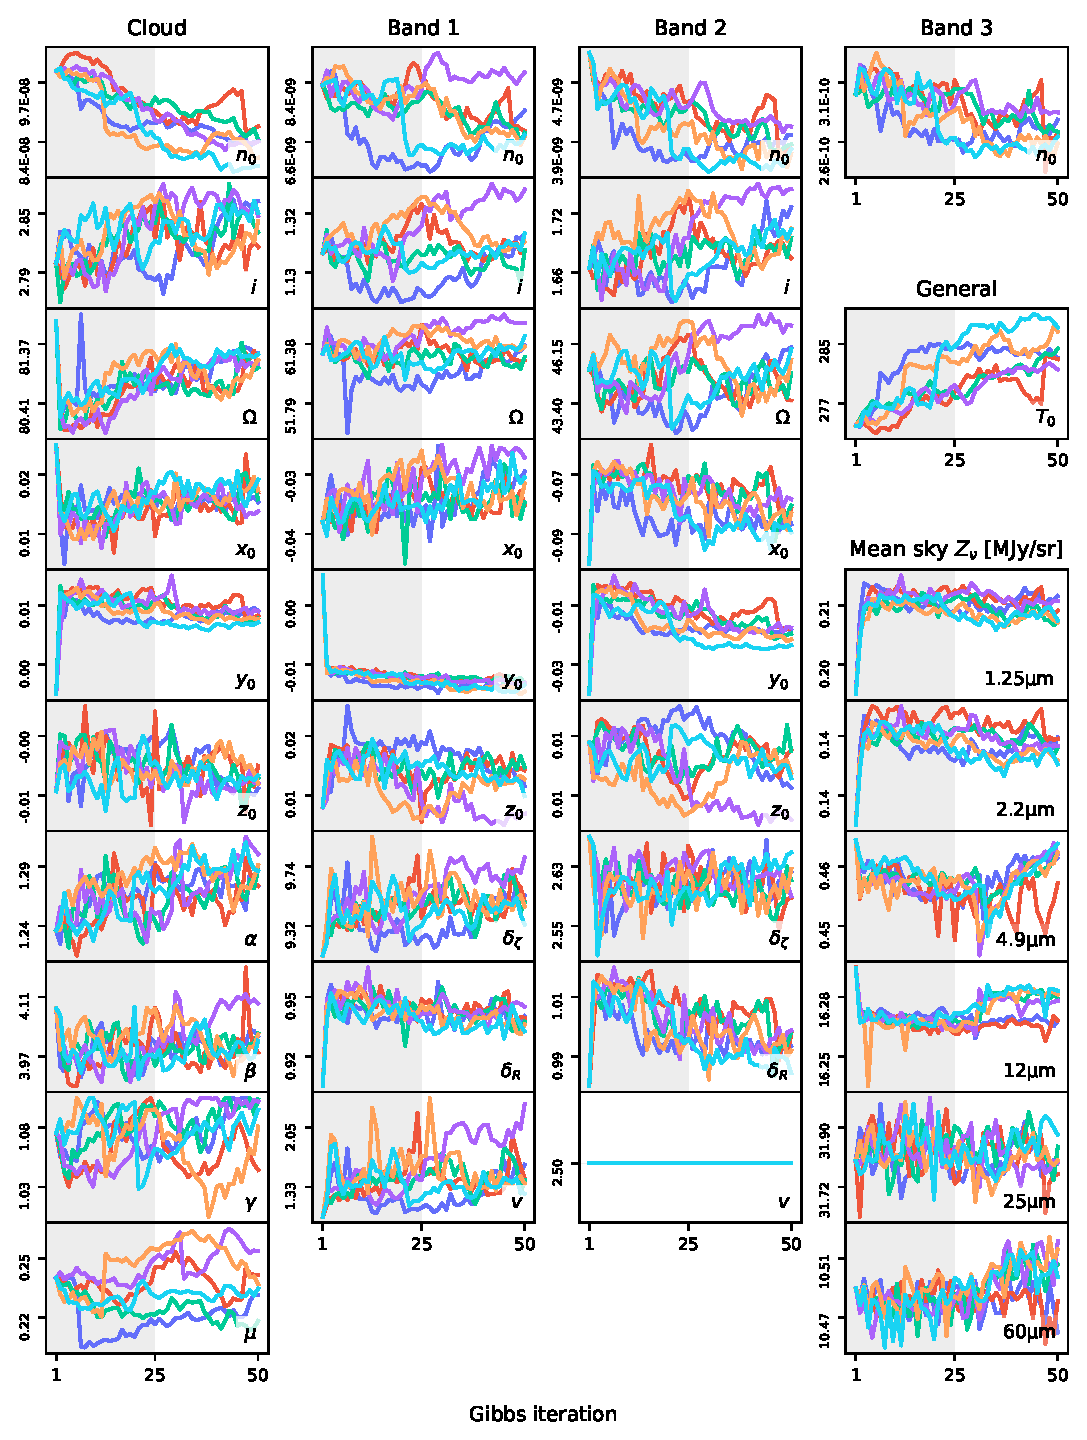
\includegraphics[width=1\textwidth]{figs/total_trace.pdf}
    \caption{Trace plot of all geometrical interplanetary dust paramteres for six independant Markov chains.}
    \label{fig:trace-ipd}
\end{figure*}

\begin{figure*}
    \centering
    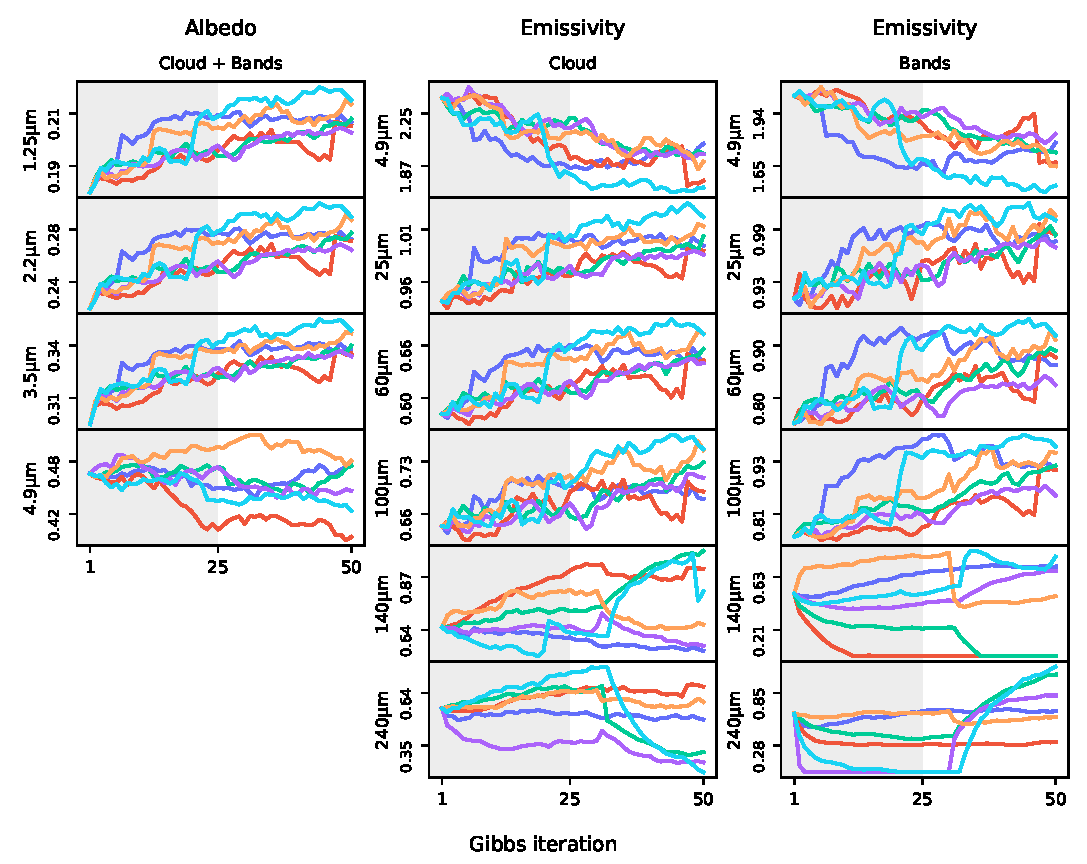
\includegraphics[width=1\textwidth]{figs/emissivity_and_albedo_trace.pdf}
    \caption{Trace plot of all geometrical interplanetary dust paramteres for six independant Markov chains.}
    \label{fig:trace-emissivity-albedo}
\end{figure*}


\subsection{Updated ZL model and goodness-of-fit}

\begin{figure}
    \centering
    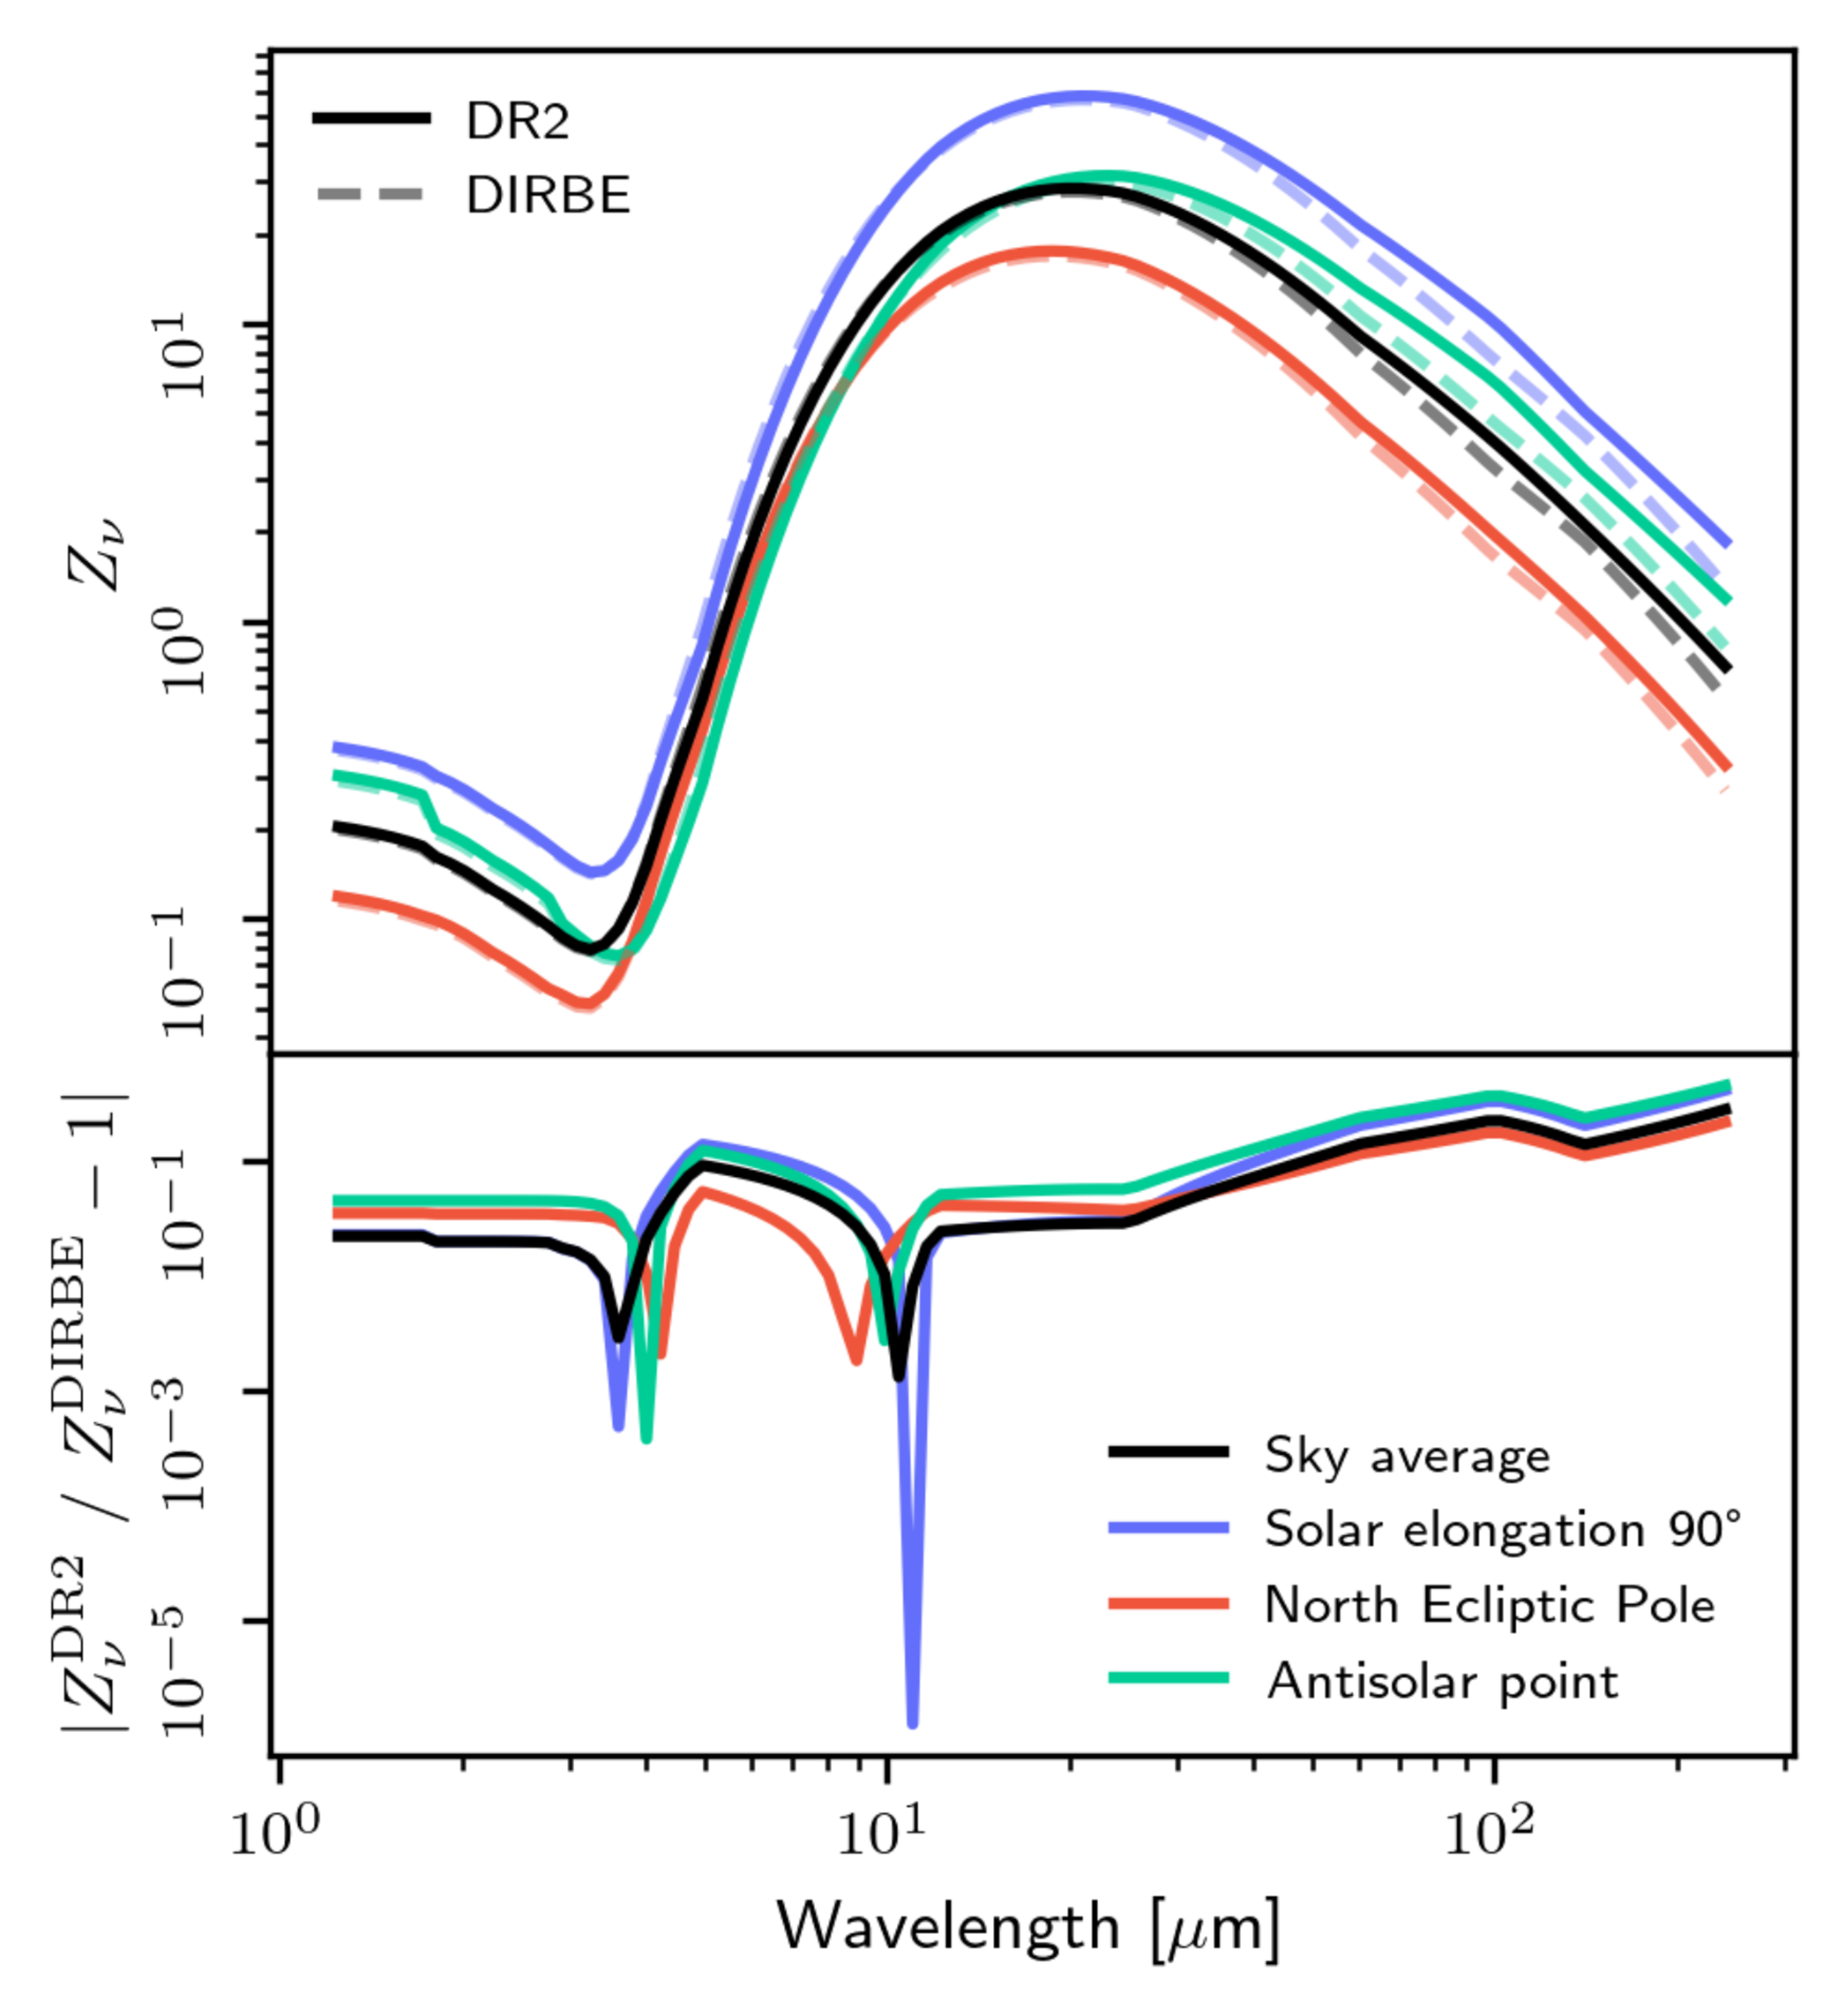
\includegraphics[width=\columnwidth]{figs/zodi_comp.pdf}
    \caption{Simulated ZL intensity on January 1, 2024 as a function of wavelength from the best-fit 
    Cosmoglobe ZL model, made with ZodiPy. The ZL SED is directional 
    and seasonal due to temperature variations along independent line-of-sights and variations in IPD composition. 
    The black curve shows the mean sky intensity in a HEALPix map with resolution
    $N_\mathrm{side}= 64$ where pixels with an angular separation of less than
    $60^\circ$ are masked out. The colored dashed lines represent the ZL 
    intensity
    }
    \label{fig:zodi-intensity}
\end{figure}

\begin{figure}
    \centering
    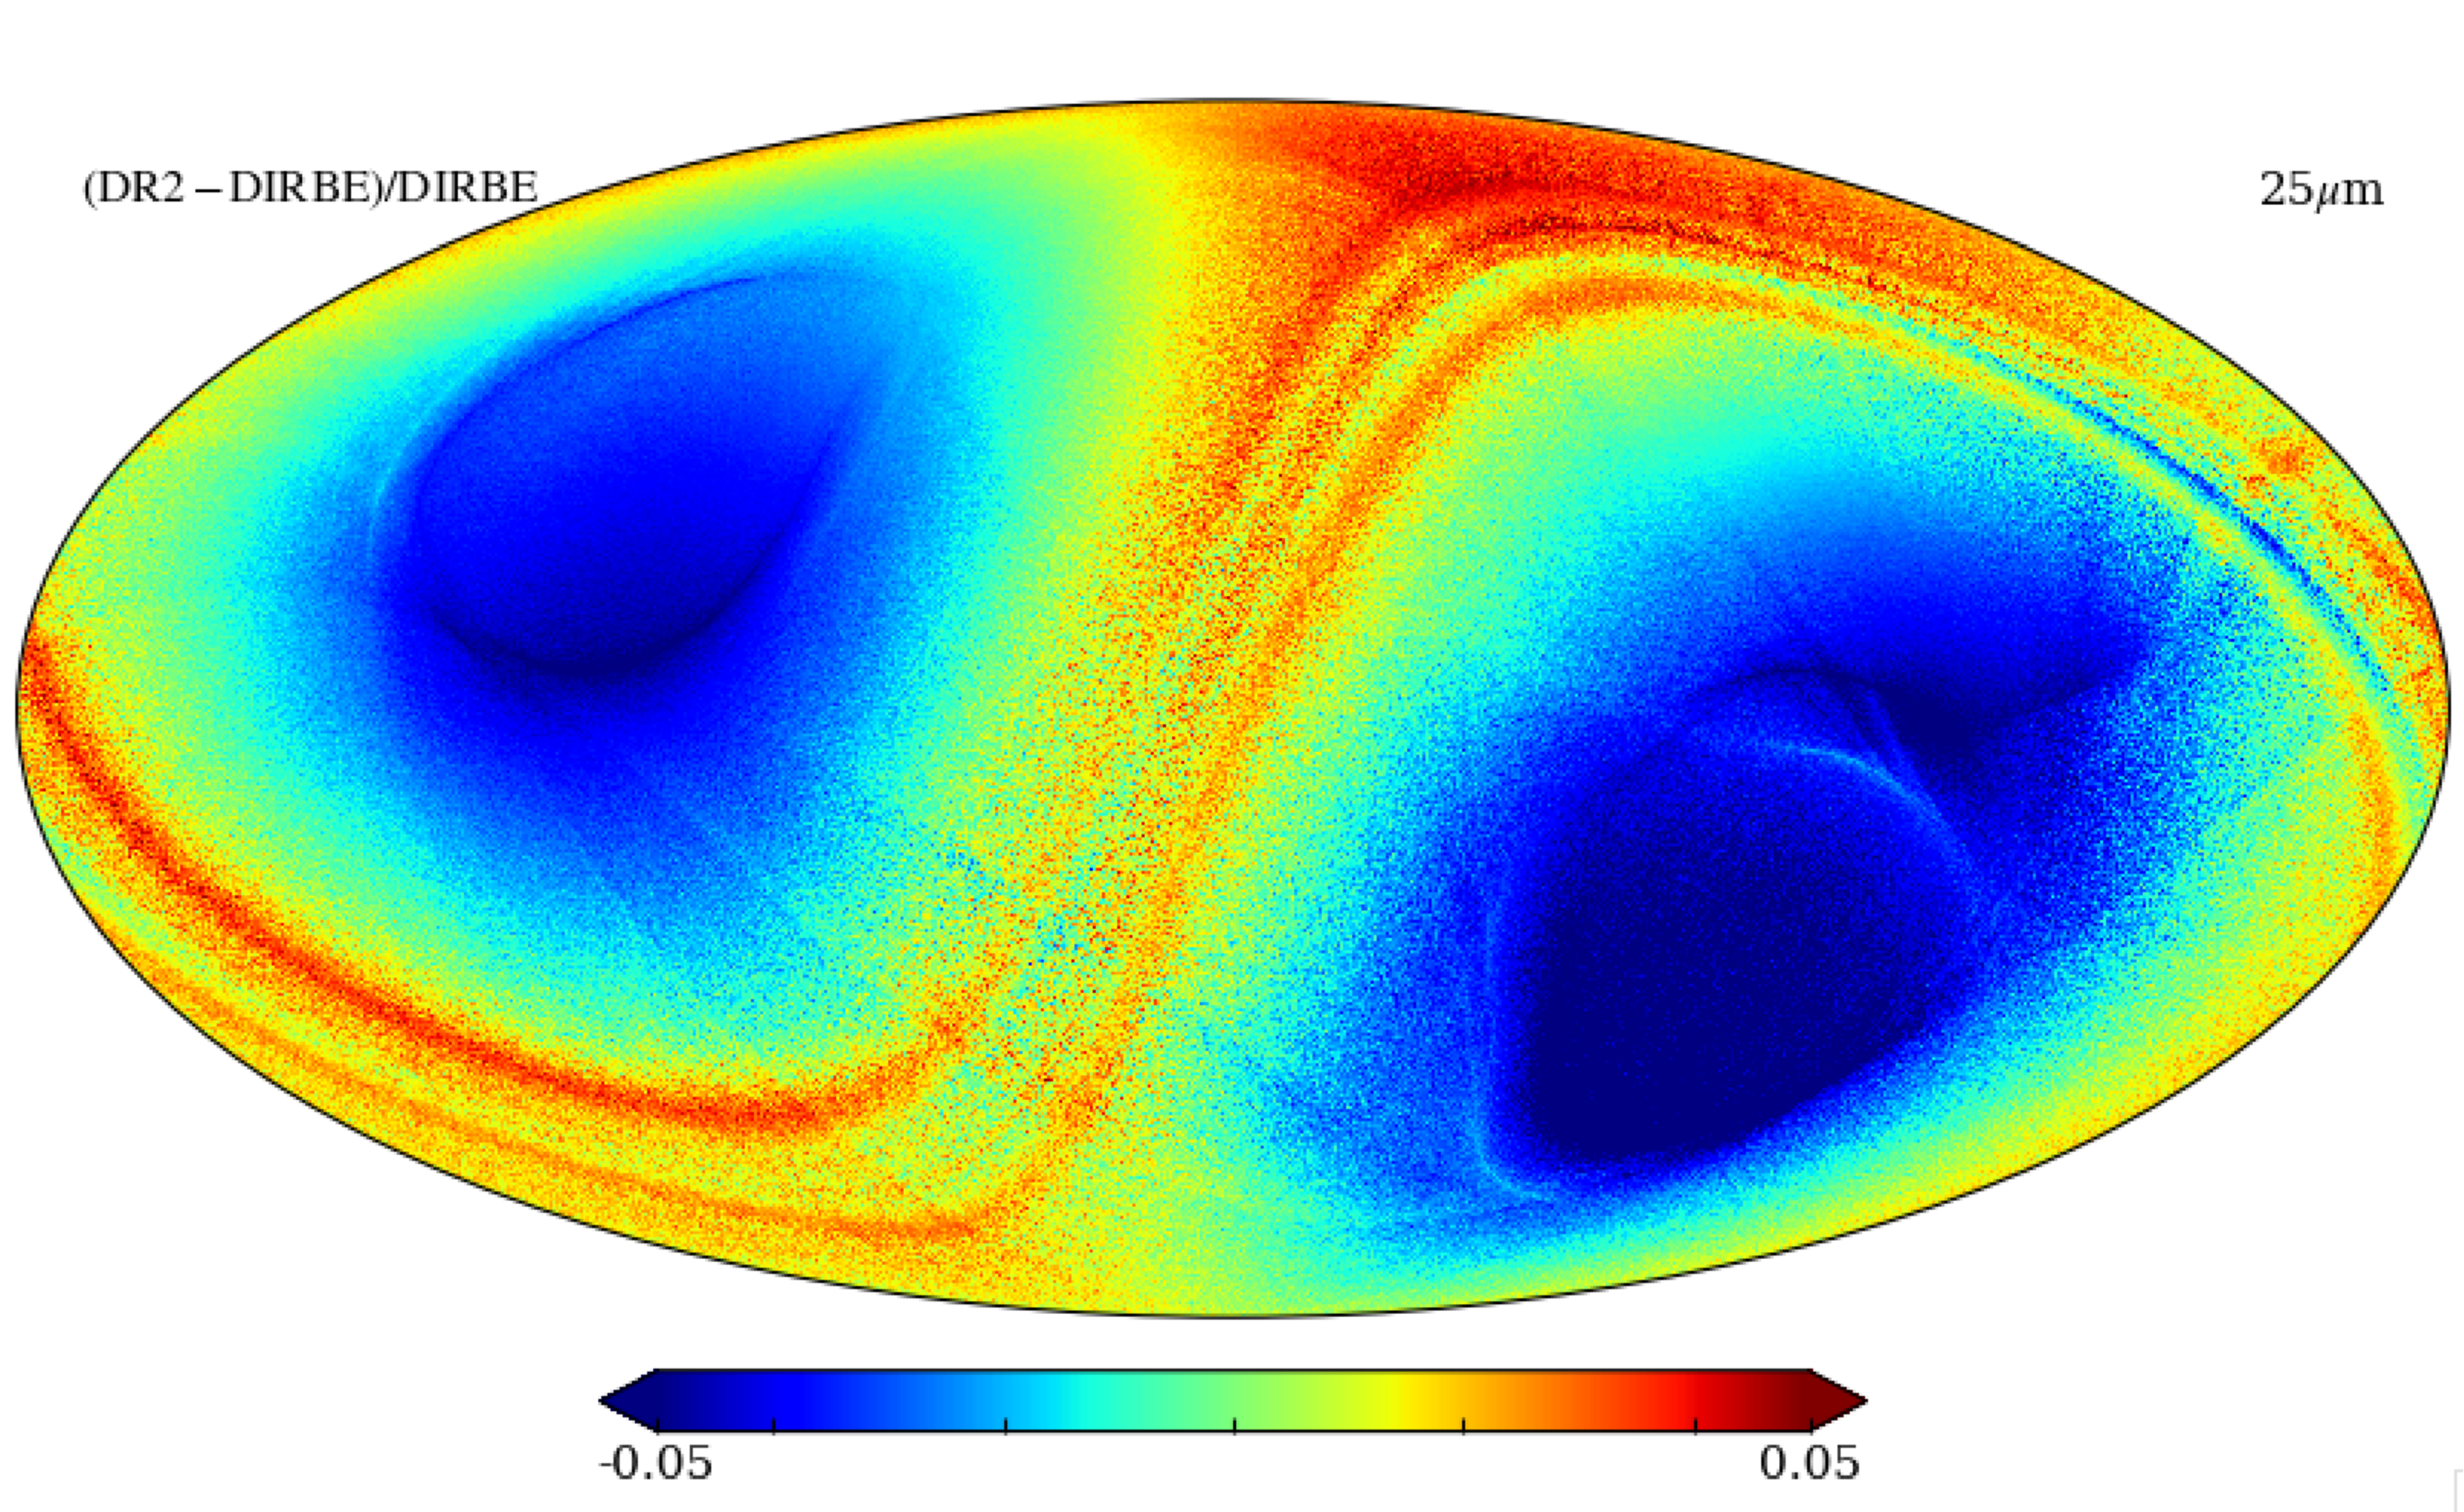
\includegraphics[width=\columnwidth]{figs/zodi_reldiff.pdf}
    \caption{}
    \label{fig:reldiff}
\end{figure}


\begin{table}
\newdimen\tblskip \tblskip=5pt
\caption{}
\label{tab:chisq}
\vskip -4mm
\footnotesize
\setbox\tablebox=\vbox{
 \newdimen\digitwidth
 \setbox0=\hbox{\rm 0}
 \digitwidth=\wd0
 \catcode`*=\active
 \def*{\kern\digitwidth}
%
  \newdimen\dpwidth
  \setbox0=\hbox{.}
  \dpwidth=\wd0
  \catcode`!=\active
  \def!{\kern\dpwidth}
%
  \halign{\hbox to 2cm{#\leaderfil}\tabskip 2em&
    \hfil$#$\hfil \tabskip 2em&
    \hfil$#$\hfil \tabskip 2em&
    \hfil$#$\hfil \tabskip 0em\cr
\noalign{\doubleline}
\omit\sc $\lambda$ ($\mu\mathrm{m}$)\hfil& N_{\mathrm{samp}} (10^3) & \sigma_{0}^{\mathrm{(a)}} [\mathrm{MJy/sr}] & \chi^2_{\mathrm{red}} \cr
\noalign{\vskip 3pt\hrule\vskip 5pt}
*1.25   & *70 & *0.031 & 0.756 \cr 
*2.2    & *51 & *0.031 & 0.770 \cr 
*3.5    & *51 & *0.026 & 1.019 \cr 
*4.9    & *99 & *0.029 & 1.150 \cr 
*12     & 225 & *0.102 & 2.649 \cr
*25     & \cdots & *0.190 & \cdots \cr 
*60     & *97 & *0.322 & 1.501 \cr 
100     & *85 & *0.381 & 1.415 \cr 
140     & 187 & 32.1*  & 1.015 \cr 
240     & 177 & 18.3*  & 1.024 \cr 
\noalign{\vskip 5pt\hrule\vskip 5pt}}}
  \endPlancktable
  \tablenote {{\rm a}} Mission average TOD noise rms per 8\,Hz sample.\par
\par
\end{table}


\begin{figure*}[t]
    \centering
    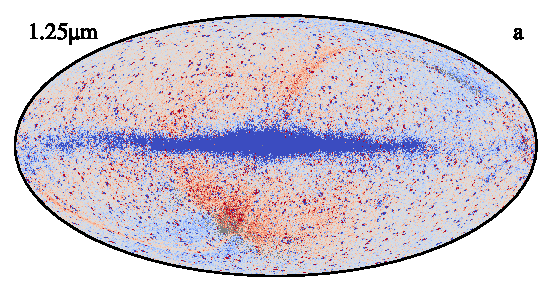
\includegraphics[width=0.22\linewidth]{figs/compare_zodi_res/cosmoglobe_res_01a.pdf}%
    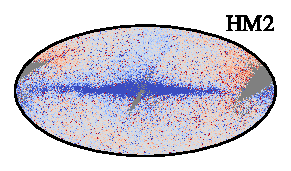
\includegraphics[width=0.22\linewidth]{figs/compare_zodi_res/cosmoglobe_res_01b.pdf}%
    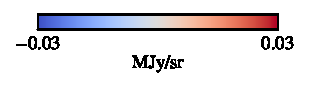
\includegraphics[width=23mm,angle=90]{figs/compare_zodi_res/cbar_01.pdf}\hspace*{3mm}
    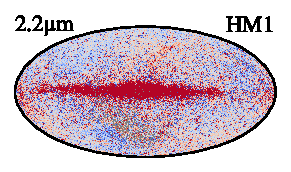
\includegraphics[width=0.22\linewidth]{figs/compare_zodi_res/cosmoglobe_res_02a.pdf}%
    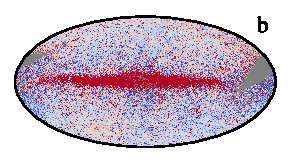
\includegraphics[width=0.22\linewidth]{figs/compare_zodi_res/cosmoglobe_res_02b.pdf}%
    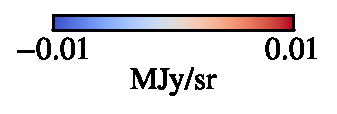
\includegraphics[width=23mm,angle=90]{figs/compare_zodi_res/cbar_02.pdf}\\
    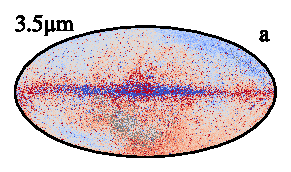
\includegraphics[width=0.22\linewidth]{figs/compare_zodi_res/cosmoglobe_res_03a.pdf}%
    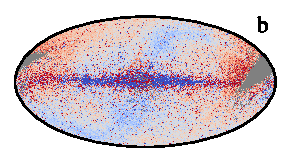
\includegraphics[width=0.22\linewidth]{figs/compare_zodi_res/cosmoglobe_res_03b.pdf}%
    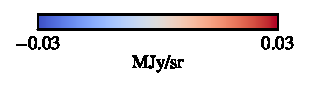
\includegraphics[width=23mm,angle=90]{figs/compare_zodi_res/cbar_03.pdf}\hspace*{3mm}
    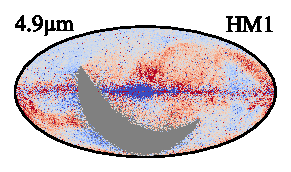
\includegraphics[width=0.22\linewidth]{figs/compare_zodi_res/cosmoglobe_res_04a.pdf}%
    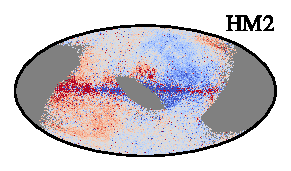
\includegraphics[width=0.22\linewidth]{figs/compare_zodi_res/cosmoglobe_res_04b.pdf}%
    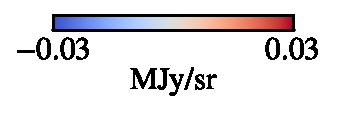
\includegraphics[width=23mm,angle=90]{figs/compare_zodi_res/cbar_04.pdf}\\
    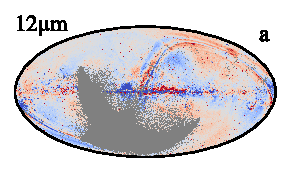
\includegraphics[width=0.22\linewidth]{figs/compare_zodi_res/cosmoglobe_res_05a.pdf}%
    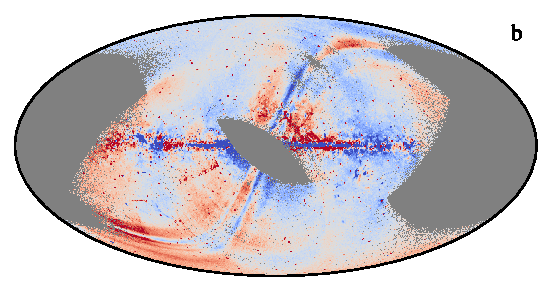
\includegraphics[width=0.22\linewidth]{figs/compare_zodi_res/cosmoglobe_res_05b.pdf}%
    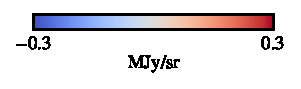
\includegraphics[width=23mm,angle=90]{figs/compare_zodi_res/cbar_05.pdf}\hspace*{3mm}
    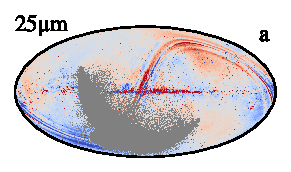
\includegraphics[width=0.22\linewidth]{figs/compare_zodi_res/cosmoglobe_res_06a.pdf}%
    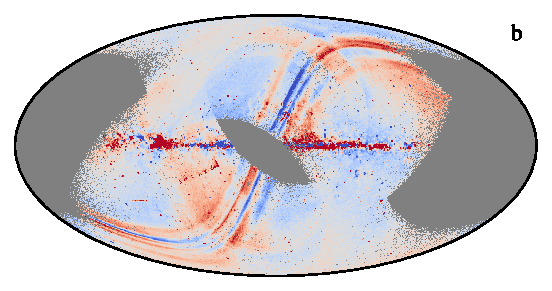
\includegraphics[width=0.22\linewidth]{figs/compare_zodi_res/cosmoglobe_res_06b.pdf}%
    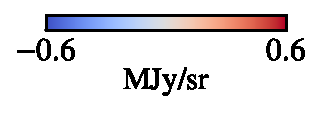
\includegraphics[width=23mm,angle=90]{figs/compare_zodi_res/cbar_06.pdf}\\
    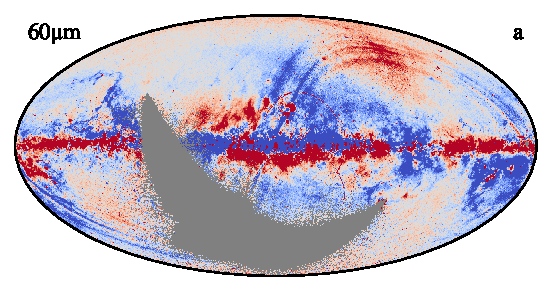
\includegraphics[width=0.22\linewidth]{figs/compare_zodi_res/cosmoglobe_res_07a.pdf}%
    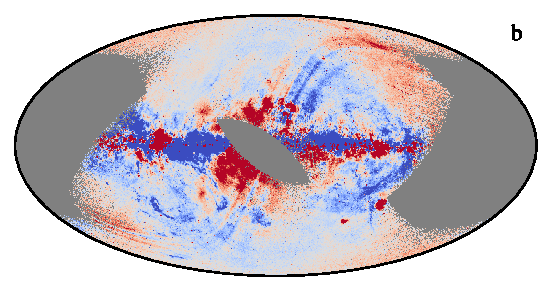
\includegraphics[width=0.22\linewidth]{figs/compare_zodi_res/cosmoglobe_res_07b.pdf}%
    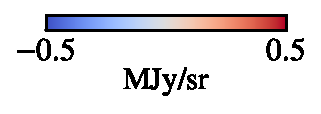
\includegraphics[width=23mm,angle=90]{figs/compare_zodi_res/cbar_07.pdf}\hspace*{3mm}
    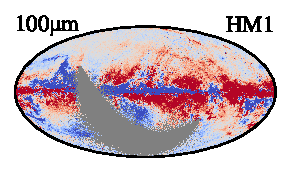
\includegraphics[width=0.22\linewidth]{figs/compare_zodi_res/cosmoglobe_res_08a.pdf}%
    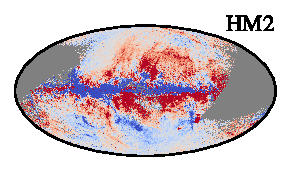
\includegraphics[width=0.22\linewidth]{figs/compare_zodi_res/cosmoglobe_res_08b.pdf}%
    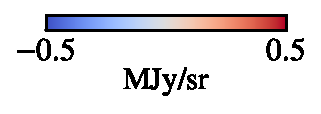
\includegraphics[width=23mm,angle=90]{figs/compare_zodi_res/cbar_08.pdf}\\
    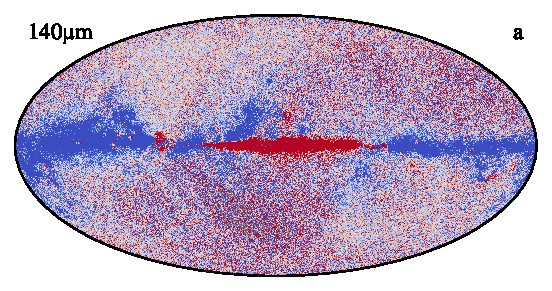
\includegraphics[width=0.22\linewidth]{figs/compare_zodi_res/cosmoglobe_res_09a.pdf}%
    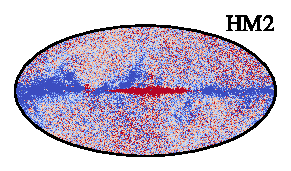
\includegraphics[width=0.22\linewidth]{figs/compare_zodi_res/cosmoglobe_res_09b.pdf}%
    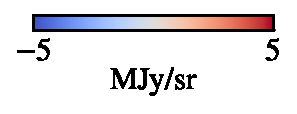
\includegraphics[width=23mm,angle=90]{figs/compare_zodi_res/cbar_09.pdf}\hspace*{3mm}
    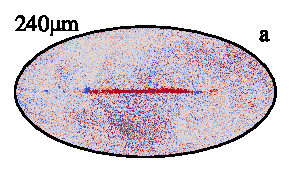
\includegraphics[width=0.22\linewidth]{figs/compare_zodi_res/cosmoglobe_res_10a.pdf}%
    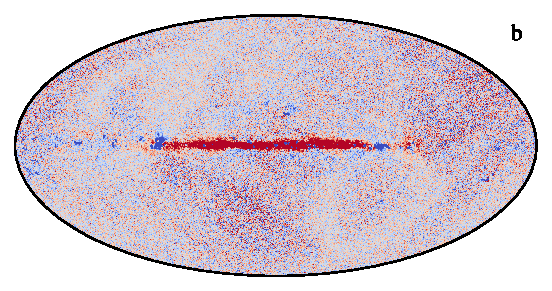
\includegraphics[width=0.22\linewidth]{figs/compare_zodi_res/cosmoglobe_res_10b.pdf}%
    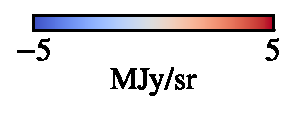
\includegraphics[width=23mm,angle=90]{figs/compare_zodi_res/cbar_10.pdf}%
    \caption{Half-mission split residual maps, smoothed by a 0.5 degrees or 15 arcmin beam.}
    \label{fig:half-mission-res2}
\end{figure*}



We illustrate the effectiveness of our model in figures~\ref{fig:dr2-zsma-compare1} 
and~\ref{fig:dr2-zsma-compare2}, which shows the data minus model residuals for both models.
We obtain cleaner residuals in all DIRBE channels with our new ZL model, most notably in the 12 and 25 $\mu$m  
ZL dominated channels.

Figure~\ref{fig:zodi-intensity} shows the interpolated ZL signal as a function of wavelength. The SED will be a composite of many independant 


\subsection{Comparison of ZSMA maps}

\textcolor{red}{(Fill in once the zodi paper gets further along and we have our results)}
\begin{figure*}
    \centering

    \resizebox{\textwidth}{!}{%
    \includegraphics[height=1cm]{figs/compare_freq_maps/cosmoglobe_ma_01.pdf}%
    \includegraphics[width=1cm,angle=90]{figs/compare_freq_maps/cbar_tot_01.pdf}%
    \includegraphics[height=1cm]{figs/compare_freq_maps/dirbe_zsma_01.pdf}%
    \includegraphics[height=1cm]{figs/compare_freq_maps/cosmoglobe_zsma_01.pdf}%
    \includegraphics[width=1cm,angle=90]{figs/compare_freq_maps/cbar_01.pdf}%
    }\\


    \resizebox{\textwidth}{!}{%
    \includegraphics[height=1cm]{figs/compare_freq_maps/cosmoglobe_ma_02.pdf}%
    \includegraphics[width=1cm,angle=90]{figs/compare_freq_maps/cbar_tot_02.pdf}%
    \includegraphics[height=1cm]{figs/compare_freq_maps/dirbe_zsma_02.pdf}%
    \includegraphics[height=1cm]{figs/compare_freq_maps/cosmoglobe_zsma_02.pdf}%
    \includegraphics[width=1cm,angle=90]{figs/compare_freq_maps/cbar_02.pdf}%
    }\\

    \resizebox{\textwidth}{!}{%
    \includegraphics[height=1cm]{figs/compare_freq_maps/cosmoglobe_ma_03.pdf}%
    \includegraphics[width=1cm,angle=90]{figs/compare_freq_maps/cbar_tot_03.pdf}%
    \includegraphics[height=1cm]{figs/compare_freq_maps/dirbe_zsma_03.pdf}%
    \includegraphics[height=1cm]{figs/compare_freq_maps/cosmoglobe_zsma_03.pdf}%
    \includegraphics[width=1cm,angle=90]{figs/compare_freq_maps/cbar_03.pdf}%
    }\\

    \resizebox{\textwidth}{!}{%
    \includegraphics[height=1cm]{figs/compare_freq_maps/cosmoglobe_ma_04.pdf}%
    \includegraphics[width=1cm,angle=90]{figs/compare_freq_maps/cbar_tot_04.pdf}%
    \includegraphics[height=1cm]{figs/compare_freq_maps/dirbe_zsma_04.pdf}%
    \includegraphics[height=1cm]{figs/compare_freq_maps/cosmoglobe_zsma_04.pdf}%
    \includegraphics[width=1cm,angle=90]{figs/compare_freq_maps/cbar_04.pdf}%
    }\\

    \resizebox{\textwidth}{!}{%
    \includegraphics[height=1cm]{figs/compare_freq_maps/cosmoglobe_ma_05.pdf}%
    \includegraphics[width=1cm,angle=90]{figs/compare_freq_maps/cbar_tot_05.pdf}%
    \includegraphics[height=1cm]{figs/compare_freq_maps/dirbe_zsma_05.pdf}%
    \includegraphics[height=1cm]{figs/compare_freq_maps/cosmoglobe_zsma_05.pdf}%
    \includegraphics[width=1cm,angle=90]{figs/compare_freq_maps/cbar_05.pdf}%
    }\\

    \resizebox{\textwidth}{!}{%
    \includegraphics[height=1cm]{figs/compare_freq_maps/cosmoglobe_ma_06.pdf}%
    \includegraphics[width=1cm,angle=90]{figs/compare_freq_maps/cbar_tot_06.pdf}%
    \includegraphics[height=1cm]{figs/compare_freq_maps/dirbe_zsma_06.pdf}%
    \includegraphics[height=1cm]{figs/compare_freq_maps/cosmoglobe_zsma_06.pdf}%
    \includegraphics[width=1cm,angle=90]{figs/compare_freq_maps/cbar_06.pdf}%
    }\\

    \resizebox{\textwidth}{!}{%
    \includegraphics[height=1cm]{figs/compare_freq_maps/cosmoglobe_ma_07.pdf}%
    \includegraphics[width=1cm,angle=90]{figs/compare_freq_maps/cbar_tot_07.pdf}%
    \includegraphics[height=1cm]{figs/compare_freq_maps/dirbe_zsma_07.pdf}%
    \includegraphics[height=1cm]{figs/compare_freq_maps/cosmoglobe_zsma_07.pdf}%
    \includegraphics[width=1cm,angle=90]{figs/compare_freq_maps/cbar_07.pdf}%
    }\\
    \caption{Comparison between ZL subtractions with our best-fit ZL model and with K98. 
    \textit{(left column):} Mission-averaged containing ZL at native HEALPix resolution 
    of $N_\mathrm{side} = 512$. \textit{(middle column):} DIRBE ZSMA maps
    at $N_\mathrm{side} = 256$.\textit{(right column):} Our ZL subtracted mission-average 
    maps, downgraded to $N_\mathrm{side} = 256$. The rows list to DIRBE frequency channels, from top to 
    bottom. We observe a clear improved ZL solution at all DIRBE channels.
    }
    \label{fig:dr2-zsma-compare1}
\end{figure*}

\begin{figure*}
    \centering
    \resizebox{\textwidth}{!}{%
    \includegraphics[height=1cm]{figs/compare_freq_maps/cosmoglobe_ma_08.pdf}%
    \includegraphics[width=1cm,angle=90]{figs/compare_freq_maps/cbar_tot_08.pdf}%
    \includegraphics[height=1cm]{figs/compare_freq_maps/dirbe_zsma_08.pdf}%
    \includegraphics[height=1cm]{figs/compare_freq_maps/cosmoglobe_zsma_08.pdf}%
    \includegraphics[width=1cm,angle=90]{figs/compare_freq_maps/cbar_08.pdf}%
    }\\

    \resizebox{\textwidth}{!}{%
    \includegraphics[height=1cm]{figs/compare_freq_maps/cosmoglobe_ma_09.pdf}%
    \includegraphics[width=1cm,angle=90]{figs/compare_freq_maps/cbar_tot_09.pdf}%
    \includegraphics[height=1cm]{figs/compare_freq_maps/dirbe_zsma_09.pdf}%
    \includegraphics[height=1cm]{figs/compare_freq_maps/cosmoglobe_zsma_09.pdf}%
    \includegraphics[width=1cm,angle=90]{figs/compare_freq_maps/cbar_09.pdf}%
    }\\

    \resizebox{\textwidth}{!}{%
    \includegraphics[height=1cm]{figs/compare_freq_maps/cosmoglobe_ma_10.pdf}%
    \includegraphics[width=1cm,angle=90]{figs/compare_freq_maps/cbar_tot_10.pdf}%
    \includegraphics[height=1cm]{figs/compare_freq_maps/dirbe_zsma_10.pdf}%
    \includegraphics[height=1cm]{figs/compare_freq_maps/cosmoglobe_zsma_10.pdf}%
    \includegraphics[width=1cm,angle=90]{figs/compare_freq_maps/cbar_10.pdf}%
    }\\

    \caption{Comparison between ZL subtractions with our best-fit ZL model and with K98. 
    \textit{(left column):} Mission-averaged containing ZL at native HEALPix resolution 
    of $N_\mathrm{side} = 512$. \textit{(middle column):} DIRBE ZSMA maps
    at $N_\mathrm{side} = 256$. The rows list to DIRBE frequency channels, from top to 
    bottom. \textit{(right column):} Our ZL subtracted mission-average 
    maps, downgraded to $N_\mathrm{side} = 256$. We observe a clear improved ZL solution at all DIRBE channels.
    }    
    \label{fig:dr2-zsma-compare2}
\end{figure*}







\begin{figure}
    \centering
    \includegraphics[width=\linewidth]{figs/zodi_mean_diff_DIRBE_DR2.pdf}
    \caption{Monopole difference between official DIRBE and
      \cosmoglobe\ DR2 ZSMA maps, evaluated as the average of the
      difference between the maps shown in the second and third
      columns in Figs.~\ref{fig:dr2-zsma-compare1} and
      \ref{fig:dr2-zsma-compare2} over the DR2 analysis masks.}
    \label{fig:zsma_mean}
\end{figure}

\begin{figure}
    \centering
    \includegraphics[width=\linewidth]{figs/zodi_rms_ratio_DIRBE_DR2_v2.pdf}
    \caption{Rms ratio between \cosmoglobe\ DR2 and DIRBE ZSMA, ,
      $\sigma_{\mathrm{DR2}}/\sigma_\mathrm{DIRBE}$,
      as evaluated outside the DR2 analysis masks.}
    \label{fig:zsma_rms}
\end{figure}



\begin{figure*}
    \centering
    \includegraphics[width=\linewidth]{figs/tod_zodi_residuals.pdf}
    \caption{}
    \label{fig:res_vs_b}
\end{figure*}


Subtracting the ZL with our best-fit-model yields lower sky residuals at all bands 
compared to the DIRBE ZSMA maps. A comparison between the ZL residuals can be seen 
in Figure~\ref{fig:dr2-zsma-compare}. Here the first column shows the frequency maps of the
four most ZL dominated DIREB bands (4.9, 12, 25, and 60 $\mu$m), the second shows the ZL
subtracted maps with our model, and column three shows the DIRBE ZSMA.




\section{Conclusions}
\label{sec:conclusions}


\begin{acknowledgements}
 The current work has received funding from the European
  Union’s Horizon 2020 research and innovation programme under grant
  agreement numbers 819478 (ERC; \textsc{Cosmoglobe}) and 772253 (ERC;
  \textsc{bits2cosmology}). Some of the results in this paper have been 
  derived using the HEALPix \citep{Gorski2005} package.
  We acknowledge the use of the Legacy Archive for Microwave Background 
  Data
  Analysis (LAMBDA), part of the High Energy Astrophysics Science
  Archive Center
  (HEASARC). HEASARC/LAMBDA is a service of the Astrophysics Science 
  Division at the NASA Goddard Space Flight Center.  
\end{acknowledgements}


%-------------------------------------------------------------
%                                       Table with references 
%-------------------------------------------------------------
%

\bibliographystyle{aa}
\bibliography{../../common/CG_bibliography,references,../../common/Planck_bib,references}
%\bibliography{references}

\appendix
\onecolumn

\section{Component-wise zodiacal light maps and number density cross-sections}
\label{sec:zodi-comps}

% \noindent\begin{minipage}{\textwidth}
In this Appendix, we present maps of visualizations of our best-fit ZL 
light model. Such figures can help illustrate the physical properties 
of the model and help validate how physical our models are. The ZL 
component-wise maps, both the mission-averaged and the instantaneous maps 
in~\ref{fig:mission-averaged-comp-maps} 
and~\ref{fig:mission-averaged-inst-maps}, respectively, are compared to 
the K98 model. The IPD number density visualization for the K98 model, 
corresponding to Figure~\ref{fig:ipd-number-density} can be seen in 
Figure~X in~\cite{San2022} .


% \end{minipage}

\begin{figure*}
    \centering
    \includegraphics[width=\textwidth]{figs/number_density.pdf}
    \caption{Visualization of the IPD number density of the four fitted zodiacal components in our model. The number densities are shown as a cross-section of the Solar system in the xz-plane. \textit{(top left):} The smooth cloud. \textit{(top right):} Dust band 1. \textit{(bottom left):} Dust band 2. \textit{(bottom right):} Dust band 3. The gray dotted line represents the ecliptic plane and helps illustrate the variations in the components symmetry planes.}
    \label{fig:ipd-number-density}
\end{figure*}


\begin{figure*}
    \centering
    \resizebox{\textwidth}{!}{%
    \includegraphics[height=1cm]{figs/comp_maps/K98_0_inst.pdf}%
    \includegraphics[height=1cm]{figs/comp_maps/CG_0_inst.pdf}%
    \includegraphics[width=1cm,angle=90]{figs/comp_maps/cbar_0_inst.pdf}%
    }\\
    \resizebox{\textwidth}{!}{%
    \includegraphics[height=1cm]{figs/comp_maps/K98_1_inst.pdf}%
    \includegraphics[height=1cm]{figs/comp_maps/CG_1_inst.pdf}%
    \includegraphics[width=1cm,angle=90]{figs/comp_maps/cbar_1_inst.pdf}%
    }\\
    \resizebox{\textwidth}{!}{%
    \includegraphics[height=1cm]{figs/comp_maps/K98_2_inst.pdf}%
    \includegraphics[height=1cm]{figs/comp_maps/CG_2_inst.pdf}%
    \includegraphics[width=1cm,angle=90]{figs/comp_maps/cbar_2_inst.pdf}%
    }\\
    \resizebox{\textwidth}{!}{%
    \includegraphics[height=1cm]{figs/comp_maps/K98_3_inst.pdf}%
    \includegraphics[height=1cm]{figs/comp_maps/CG_3_inst.pdf}%
    \includegraphics[width=1cm,angle=90]{figs/comp_maps/cbar_3_inst.pdf}%
    }\\
    \caption{Full-sky component-wise ZL maps (January 1, 2024) at $25\mu$m made with ZodiPy. 
    \textit{(left column:)} The K98 model. \textit{(right column:)} Best-fit Cosmoglobe ZL model. 
    Rows list the zodiacal components, from top to bottom, 1) smooth cloud; 2) dust band 1; 3) 
    dust band 2; 4) dust band 3. The maps are in ecliptic coordinates, with the Sun marked as 
    an orange circle.}
    \label{fig:mission-averaged-inst-maps}
\end{figure*}

\begin{figure*}[hbt]
    \centering
    \resizebox{\textwidth}{!}{%
    \includegraphics[height=1cm]{figs/comp_maps/K98_0.pdf}%
    \includegraphics[height=1cm]{figs/comp_maps/DR2_0.pdf}%
    \includegraphics[width=1cm,angle=90]{figs/comp_maps/cbar_0.pdf}%
    }\\
    \resizebox{\textwidth}{!}{%
    \includegraphics[height=1cm]{figs/comp_maps/K98_1.pdf}%
    \includegraphics[height=1cm]{figs/comp_maps/DR2_1.pdf}%
    \includegraphics[width=1cm,angle=90]{figs/comp_maps/cbar_1.pdf}%
    }\\
    \resizebox{\textwidth}{!}{%
    \includegraphics[height=1cm]{figs/comp_maps/K98_2.pdf}%
    \includegraphics[height=1cm]{figs/comp_maps/DR2_2.pdf}%
    \includegraphics[width=1cm,angle=90]{figs/comp_maps/cbar_2.pdf}%
    }\\
    \resizebox{\textwidth}{!}{%
    \includegraphics[height=1cm]{figs/comp_maps/K98_3.pdf}%
    \includegraphics[height=1cm]{figs/comp_maps/DR2_3.pdf}%
    \includegraphics[width=1cm,angle=90]{figs/comp_maps/cbar_3.pdf}%
    }\\
    \caption{Mission-averaged component-wise ZL maps at $25\mu$m made with ZodiPy. 
    \textit{(left column:)} The K98 model. \textit{(right column:)} Best-fit Cosmoglobe ZL model.
    Rows list the zodiacal components, from top to bottom, 1) smooth cloud; 2) dust band 1; 3) 
    dust band 2; 4) dust band 3. The maps are in galactic coordinates.}
    \label{fig:mission-averaged-comp-maps}
\end{figure*}

\clearpage

\section{Interplanetary dust parameter atlas}
\label{sec:param-atlas}
In this Appendix, we present an atlas of mission-averaged ZL parameter maps.
Each map represents the effect of changing one ZL model parameter by $\pm 5\%$ while holding the other fixed. The maps are normalized.

\begin{figure*}[hbt]
    \centering
    \resizebox{0.82\textwidth}{!}{%
    \includegraphics[height=1cm]{figs/atlas/C_01.pdf}%
    \includegraphics[height=1cm]{figs/atlas/B1_01.pdf}%
    \includegraphics[height=1cm]{figs/atlas/B2_01.pdf}%
    \includegraphics[height=1cm]{figs/atlas/B3_01.pdf}%
    }\\
    \resizebox{0.82\textwidth}{!}{%
    \includegraphics[height=1cm]{figs/atlas/C_02.pdf}%
    \includegraphics[height=1cm]{figs/atlas/B1_02.pdf}%
    \includegraphics[height=1cm]{figs/atlas/B2_02.pdf}%
    \includegraphics[height=1cm]{figs/atlas/B3_02.pdf}%
    }\\
    \resizebox{0.82\textwidth}{!}{%
    \includegraphics[height=1cm]{figs/atlas/C_03.pdf}%
    \includegraphics[height=1cm]{figs/atlas/B1_03.pdf}%
    \includegraphics[height=1cm]{figs/atlas/B2_03.pdf}%
    \includegraphics[height=1cm]{figs/atlas/B3_03.pdf}%
    }\\
    \resizebox{0.82\textwidth}{!}{%
    \includegraphics[height=1cm]{figs/atlas/C_04.pdf}%
    \includegraphics[height=1cm]{figs/atlas/B1_04.pdf}%
    \includegraphics[height=1cm]{figs/atlas/B2_04.pdf}%
    \includegraphics[height=1cm]{figs/atlas/B3_04.pdf}%
    }\\
    \resizebox{0.82\textwidth}{!}{%
    \includegraphics[height=1cm]{figs/atlas/C_05.pdf}%
    \includegraphics[height=1cm]{figs/atlas/B1_05.pdf}%
    \includegraphics[height=1cm]{figs/atlas/B2_05.pdf}%
    \includegraphics[height=1cm]{figs/atlas/B3_05.pdf}%
    }\\
    \resizebox{0.82\textwidth}{!}{%
    \includegraphics[height=1cm]{figs/atlas/C_06.pdf}%
    \includegraphics[height=1cm]{figs/atlas/B1_06.pdf}%
    \includegraphics[height=1cm]{figs/atlas/B2_06.pdf}%
    \includegraphics[height=1cm]{figs/atlas/B3_06.pdf}%
    }\\
    \resizebox{0.82\textwidth}{!}{%
    \includegraphics[height=1cm]{figs/atlas/C_07.pdf}%
    \includegraphics[height=1cm]{figs/atlas/B1_07.pdf}%
    \includegraphics[height=1cm]{figs/atlas/B2_07.pdf}%
    \includegraphics[height=1cm]{figs/atlas/B3_07.pdf}%
    }\\
    \resizebox{0.82\textwidth}{!}{%
    \includegraphics[height=1cm]{figs/atlas/C_08.pdf}%
    \includegraphics[height=1cm]{figs/atlas/B1_08.pdf}%
    \includegraphics[height=1cm]{figs/atlas/B2_08.pdf}%
    \includegraphics[height=1cm]{figs/atlas/B3_08.pdf}%
    }\\
    \resizebox{0.82\textwidth}{!}{%
    \includegraphics[height=1cm]{figs/atlas/C_09.pdf}%
    \includegraphics[height=1cm]{figs/atlas/B1_09.pdf}%
    \includegraphics[height=1cm]{figs/atlas/B2_09.pdf}%
    \includegraphics[height=1cm]{figs/atlas/B3_09.pdf}%
    }\\
    \resizebox{0.82\textwidth}{!}{%
    \includegraphics[height=1cm]{figs/atlas/C_10.pdf}%
    \includegraphics[height=1cm]{figs/atlas/B1_10.pdf}%
    \includegraphics[height=1cm]{figs/atlas/B2_10.pdf}%
    \includegraphics[height=1cm]{figs/atlas/B3_10.pdf}%
    }\\
   
    \caption{ZL parameter atlas showing the difference between increasing 
    and lowering each ZL model parameter by $5\%$ in the form of normalized 
    mission-averaged ZL maps. Columns list, from left to right parameters of
    1) the smooth cloud; 2) dust band 1; 3) dust band 2; and 4) dust band 3.}
    \label{fig:atlas1}
\end{figure*}
\begin{figure*}
    \centering
    \resizebox{0.82\textwidth}{!}{%
    \includegraphics[height=1cm]{figs/atlas/SR_01.pdf}%
    \includegraphics[height=1cm]{figs/atlas/SR_06.pdf}%
    \includegraphics[height=1cm]{figs/atlas/TF_01.pdf}%
    \includegraphics[height=1cm]{figs/atlas/TF_06.pdf}%
    }\\   
    \resizebox{0.82\textwidth}{!}{%
    \includegraphics[height=1cm]{figs/atlas/SR_02.pdf}%
    \includegraphics[height=1cm]{figs/atlas/SR_07.pdf}%
    \includegraphics[height=1cm]{figs/atlas/TF_02.pdf}%
    \includegraphics[height=1cm]{figs/atlas/TF_07.pdf}%
    }\\
    \resizebox{0.82\textwidth}{!}{%
    \includegraphics[height=1cm]{figs/atlas/SR_03.pdf}%
    \includegraphics[height=1cm]{figs/atlas/SR_08.pdf}%
    \includegraphics[height=1cm]{figs/atlas/TF_03.pdf}%
    \includegraphics[height=1cm]{figs/atlas/TF_08.pdf}%
    }\\
    \resizebox{0.82\textwidth}{!}{%
    \includegraphics[height=1cm]{figs/atlas/SR_04.pdf}%
    \includegraphics[height=1cm]{figs/atlas/SR_09.pdf}%
    \includegraphics[height=1cm]{figs/atlas/TF_04.pdf}%
    \includegraphics[height=1cm]{figs/atlas/TF_09.pdf}%
    }\\
    \resizebox{0.82\textwidth}{!}{%
    \includegraphics[height=1cm]{figs/atlas/SR_05.pdf}%
    \includegraphics[height=1cm]{figs/atlas/TF_05.pdf}%
    \includegraphics[height=1cm]{figs/atlas/TF_10.pdf}%
    \includegraphics[height=1cm]{figs/atlas/TF_11.pdf}%
    }\\
    \resizebox{0.41\textwidth}{!}{%
    \includegraphics[height=1cm]{figs/atlas/general_01.pdf}%
    \includegraphics[height=1cm]{figs/atlas/general_02.pdf}%
    }
    %\hspace*{0.47\textwidth}
    \caption{ZL parameter atlas showing the difference between increasing 
    and lowering each ZL model parameter by $5\%$ in the form of normalized 
    mission-averaged ZL maps. Columns list, from left to right parameters of
    1) the smooth cloud; 2) dust band 1; 3) dust band 2; and 4) dust band 3.}
    \label{fig:atlas2}
\end{figure*}




\end{document}
%%%% End of aa.dem
